%%%%%%%%%%%%%%%%%%%%%%%%%%%%%%%%%%%%%%%%%%%%%%%%%%%%%%%%%%%%%%%%%%%%%%%%
% Uni Duesseldorf
% Lehrstuhl fuer Datenbanken und Informationssysteme
% Vorlage fuer Bachelor-/Masterarbeiten
% Optimiert fuer den Original-Latex-Kompiler LATEX.EXE (LaTeX=>PS=>PDF)
%%%%%%%%%%%%%%%%%%%%%%%%%%%%%%%%%%%%%%%%%%%%%%%%%%%%%%%%%%%%%%%%%%%%%%%%
% Ueberarbeitung für pdflatex (LaTeX=>PDF)
%%%%%%%%%%%%%%%%%%%%%%%%%%%%%%%%%%%%%%%%%%%%%%%%%%%%%%%%%%%%%%%%%%%%%%%%
% Vorlage Changelog:
% 10.09.2015 (Matthias Liebeck): Nummerierung des Inhaltsverzeichnis nun römisch, Beispiel für einen Anhang eingebaut, \raggedbottom hinter sections eingefügt
% 11.07.2018 (Matthias Liebeck): Ersetzung des Bibliographiestils, Einsatz von Biber
% 04.09.2018 (Matthias Liebeck):
%   * Bibtex: unnötige Bibtexfelder beim Rendern ausblenden (thx @ Markus Brenneis)
%   * ngerman: "et al." im BibTeX für drei oder mehr Autoren
%   * Neuer Befehl \sectionforcestartright: Sections immer rechts beginnen (thx @ Philipp Grawe)
%   * ngerman: Deutsche Anführungszeichen im Literaturverzeichnis (thx @ Markus Brenneis)
%   * ngerman: Deutsche Anführungszeichen im Literaturverzeichnis (thx @ Markus Brenneis)
% 16.10.2018 (Matthias Liebeck): Zwei fixes an \sectionforcestartright (thx @ Markus Brenneis)
%%%%%%%%%%%%%%%%%%%%%%%%%%%%%%%%%%%%%%%%%%%%%%%%%%%%%%%%%%%%%%%%%%%%%%%%
%%%% BEGINN EINSTELLUNG FUER DIE ARBEIT. UNBEDINGT ERFORDERLICH! %%%%%%%
%%%%%%%%%%%%%%%%%%%%%%%%%%%%%%%%%%%%%%%%%%%%%%%%%%%%%%%%%%%%%%%%%%%%%%%%
% Geben Sie Ihren Namen hier an:

\newcommand{\bearbeiter}{Markus Stroh}

% Geben Sie hier den Titel Ihrer Arbeit an:
\newcommand{\titel}{Analyse des Kundenverhaltens durch Mustererkennung in Logfiles}

% Geben Sie das Datum des Beginns und Ende der Bachelorarbeit ein:
\newcommand{\beginndatum}{18. Februar 2020}
\newcommand{\abgabedatum}{18.~Mai~2020}

% Geben Sie die Namen des Erst- und Zweitgutachters an:
\newcommand{\erstgutachter}{Prof. Dr.~Stefan Conrad}
\newcommand{\zweitgutachter}{Prof. Dr.~Stefan Conrad}

% Falls Sie die Arbeit zweiseitig ausdrucken wollen,
% benutzen Sie die folgende Zeile mit
% \AN fuer zweiseitigen Druck
% \AUS fuer einseitigen Druck
\newcommand{\zweiseitig}{\AN}
% true fuer biber, false fuer klassischen Zitierstil
%\newcommand{\biber}{false}
\newcommand{\biber}{true}

% Falls Sections immer rechts beginnen sollen. Gerade für Masterarbeiten
% interessant. Bei kurzen Bachelorarbeiten eher weniger zu verwenden.
\newcommand{\sectionforcestartright}{false}
%\newcommand{\sectionforcestartright}{true}

% Falls die Arbeit in englischer Sprache verfasst
% werden soll, dann benutzen Sie die folgende Zeile mit
% englisch fuer englische Sprache
% deutsch fuer deutsche Sprache
\newcommand{\sprache}{deutsch}

% Hier wird eingestellt, ob es sich bei der Arbeit um eine Bachelor-
% oder Masterarbeit handelt (unpassendes auskommentieren!):
\newcommand{\arbeit}{Bachelorarbeit}
%~ \newcommand{\arbeit}{Masterarbeit}


%%%%%%%%%%%%%%%%%%%%%%%%%%%%%%%%%%%%%%%%%%%%%%%%%%%%%%%%%%%%%%%%%%%%%%%%
%%%% ENDE EINSTELLUNGEN %%%%%%%%%%%%%%%%%%%%%%%%%%%%%%%%%%%%%%%%%%%%%%%%
%%%%%%%%%%%%%%%%%%%%%%%%%%%%%%%%%%%%%%%%%%%%%%%%%%%%%%%%%%%%%%%%%%%%%%%%

% Die folgende Zeile NICHT EDITIEREN oder loeschen


%%%%%%%%%%%%%%%%%%%%%%%%%%%%%%%%%%%%%%%%%%%%%%%%%%%%%%%%%%%
% Obere Titelmakros. Editieren Sie diese Datei nur, wenn
% Sie sich ABSOLUT sicher sind, was Sie da tun!!!
% (Z.B. zum Abaendern der BA-Vorlage in eine MA-Vorlage)
% Uni Duesseldorf
% Lehrstuhl fuer Datenbanken und Informationssysteme
% Version 2.2 - 2.3.2010
%%%%%%%%%%%%%%%%%%%%%%%%%%%%%%%%%%%%%%%%%%%%%%%%%%%%%%%%%%%
\newcommand{\AN}{twoside}
\newcommand{\AUS}{}


%\newcommand{\englisch}{}
%\newcommand{\deutsch}{\usepackage[german]{babel}}

%% Die folgenden auskommentierten Optionen dienen der automatischen
%% Erkennung des Latex-Kompilers und dem Setzen der davon abhängigen
%% Einstellungen. Bei Problem z.B. mit dem Einbinden von verschiedenen
%% Grafiktypen bei Verwendung von PdfLatex oder Latex, einfach die
%% verschiedenen \usepackage(s) ausprobieren. (Mit diesen Einstellungen
%% funktionierte diese Vorlage bei der Verwenundg von latex.exe als
%% Kompiler bei den meisten Studierenden.)

%\newif\ifpdf \ifx\pdfoutput\undefined
%\pdffalse % we are not running pdflatex
%\else
%\pdfoutput=1 % we are running pdflatex
%\pdfcompresslevel=9 % compression level for text and image;
%\pdftrue \fi

\documentclass[11pt,a4paper, \zweiseitig]{article}
\usepackage{ifthen}


%\usepackage[iso]{umlaute}
\usepackage[utf8]{inputenc}
\usepackage{palatino} % palatino Schriftart
%\usepackage{makeidx} % um ein Index zu erstellen
\usepackage[nottoc]{tocbibind}
\usepackage[T1]{fontenc} %fuer richtige Trennung bei Umlauten
\usepackage{fancybox} % fuer die Rahmen
\usepackage{shortvrb}
\usepackage{url}
\usepackage{verbatim} 
\usepackage{xcolor}
\usepackage[colorlinks,citecolor=blue,linkcolor=black]{hyperref} %anklickbares Inhaltsverzeichnis

\ifthenelse{\boolean{\biber}}{
	% only needed for biber
	\usepackage[style=authoryear,natbib=true,backend=biber,mincitenames=1,maxcitenames=2,maxbibnames=99,uniquelist=false,dashed=false]{biblatex}
	
	% https://tex.stackexchange.com/a/334703/8850
	\AtEveryBibitem{%
	  \clearfield{issn}
	  \clearfield{isbn}
	  \clearfield{doi}
	  \clearfield{location}
	  \clearlist{location}
	  \clearlist{address}
	
	  \ifentrytype{online}{}{% Remove url except for @online
	    \clearfield{url}
	  }
	}
}
{}%no else

% Falls es bei \citet ein Komma zwischen Name und Jahr gibt:
% https://tex.stackexchange.com/questions/312539/unwanted-comma-between-author-and-year-using-citet-command
% (thx @ Markus Brenneis)
%\DeclareDelimFormat[cbx@textcite]{nameyeardelim}{\addspace}



\ifthenelse{\equal{\sprache}{deutsch}}{
 \usepackage[ngerman]{babel}
 % Bibtex u.a -> et al.
 \ifthenelse{\boolean{\biber}}{
	 \DefineBibliographyStrings{ngerman}{
	   andothers = {{et\,al\adddot}},
	 }
 \newcommand{\references}{Literatur}
 }
 	{} % do nothing when not using biber
 \usepackage[autostyle, german=quotes]{csquotes} % Deutsche Anführungszeichen im Literaturverzeichnis (thx @ Markus Brenneis)
 
 }{ \newcommand{\references}{References}}

\usepackage{a4wide} % ganze A4 Weite verwenden



%\ifpdf
%\usepackage[pdftex,xdvi]{graphicx}
%\usepackage{thumbpdf} %thumbs fuer Pdf
%\usepackage[pdfstartview=FitV]{hyperref} %anklickbares Inhaltsverzeichnis
%\else
%\usepackage[dvips,xdvi]{graphicx}
\usepackage{graphicx}

%\fi

\newcommand{\redt}[1] {
  \textcolor{red}{#1}}

\newcommand{\oranget}[1] {
  \textcolor{orange}{#1}}

\newcommand{\purplet}[1] {
  \textcolor{purple}{#1}}

%%%%%%%%%%%%%%%%%%%%%%% Massangaben fuer die Arbeit %%%%%%%%%%%%%%%
\setlength{\textwidth}{15cm}

\setlength{\oddsidemargin}{35mm}
\setlength{\evensidemargin}{25mm}

\addtolength{\oddsidemargin}{-1in}
\addtolength{\evensidemargin}{-1in}

\ifthenelse{\boolean{\biber}}{\addbibresource{references.bib}}{}

%\makeindex

\begin{document}

%\setcounter{secnumdepth}{4} %Nummerieren bis in die 4. Ebene
%\setcounter{tocdepth}{4} %Inhaltsverzeichnis bis zur 4. Ebene

\pagestyle{headings}

\sloppy % LaTeX ist dann nicht so streng mit der Silbentrennung
%~ \MakeShortVerb{\§}

\parindent0mm
\parskip0.5em


{
\textwidth170mm 
\oddsidemargin30mm 
\evensidemargin30mm 
\addtolength{\oddsidemargin}{-1in}
\addtolength{\evensidemargin}{-1in}

\parskip0pt plus2pt

% Die Raender muessen eventuell fuer jeden Drucker individuell eingestellt
% werden. Dazu sind die Werte fuer die Abstaende `\oben' und `\links' zu
% aendern, die von mir auf jeweils 0mm eingestellt wurden.

%\newlength{\links} \setlength{\links}{10mm}  % hier abzuaendern
%\addtolength{\oddsidemargin}{\links}
%\addtolength{\evensidemargin}{\links}

\begin{titlepage}
\vspace*{-1.5cm}
  \raisebox{17mm}{
    \begin{minipage}[t]{70mm}
      \begin{center}
        %\selectlanguage{german}
        {\Large INSTITUT FÜR INFORMATIK\\}
        {\normalsize
          Datenbanken und Informationssysteme\\
        }
        \vspace{3mm}
        {\small Universitätsstr. 1 \hspace{5ex} D--40225 Düsseldorf\\}
     \end{center}
    \end{minipage}
  }
  \hfill
  \raisebox{7mm}{
  
\includegraphics[width=130pt]{bilder/HHU_Logo}}
  \vspace{14em}

% Titel
  \begin{center}
      	\baselineskip=55pt
    	\textbf{\huge \titel}
  	 	\baselineskip=0 pt
   \end{center}

  %\vspace{7em}

\vfill

% Autor
  \begin{center}
    \textbf{\Large
      \bearbeiter
    }
  \end{center}

  \vspace{35mm}
 
% Prüfungsordnungs-Angaben
  \begin{center}
    %\selectlanguage{german}
    
%%%%%%%%%%%%%%%%%%%%%%%%%%%%%%%%%%%%%%%%%%%%%%%%%%%%%%%%%%%%%%%%%%%%%%%%%
% Ja, richtig, hier kann die BA-Vorlage zur MA-Vorlage gemacht werden...
% (nicht mehr nötig!)
%%%%%%%%%%%%%%%%%%%%%%%%%%%%%%%%%%%%%%%%%%%%%%%%%%%%%%%%%%%%%%%%%%%%%%%%%
    {\Large \arbeit}

    \vspace{2em}

    \begin{tabular}[t]{ll}
      Beginn der Arbeit:& \beginndatum \\
      Abgabe der Arbeit:& \abgabedatum \\
      Gutachter:         & \erstgutachter \\
                         & \zweitgutachter \\
    \end{tabular}
  \end{center}

\end{titlepage}

}

%%%%%%%%%%%%%%%%%%%%%%%%%%%%%%%%%%%%%%%%%%%%%%%%%%%%%%%%%%%%%%%%%%%%%
\clearpage
\begin{titlepage}
  ~                % eine leere Seite hinter dem Deckblatt
\end{titlepage}
%%%%%%%%%%%%%%%%%%%%%%%%%%%%%%%%%%%%%%%%%%%%%%%%%%%%%%%%%%%%%%%%%%%%%
\clearpage
\begin{titlepage}
\vspace*{\fill}

\section*{Erklärung}

%%%%%%%%%%%%%%%%%%%%%%%%%%%%%%%%%%%%%%%%%%%%%%%%%%%%%%%%%%%
% Und hier ebenfalls ggf. BA durch MA ersetzen...
% (Auch nicht mehr nötig!)
%%%%%%%%%%%%%%%%%%%%%%%%%%%%%%%%%%%%%%%%%%%%%%%%%%%%%%%%%%%

Hiermit versichere ich, dass ich diese \arbeit{}
selbstständig verfasst habe. Ich habe dazu keine anderen als die
angegebenen Quellen und Hilfsmittel verwendet.

\vspace{25 mm}

\begin{tabular}{lc}
Düsseldorf, den \abgabedatum \hspace*{2cm} & \underline{\hspace{6cm}}\\
& \bearbeiter
\end{tabular}

\vspace*{\fill}
\end{titlepage}

%%%%%%%%%%%%%%%%%%%%%%%%%%%%%%%%%%%%%%%%%%%%%%%%%%%%%%%%%%%%%%%%%%%%%
% Leerseite bei zweiseitigem Druck
%%%%%%%%%%%%%%%%%%%%%%%%%%%%%%%%%%%%%%%%%%%%%%%%%%%%%%%%%%%%%%%%%%%%%

\ifthenelse{\equal{\zweiseitig}{twoside}}{\clearpage\begin{titlepage}
~\end{titlepage}}{}

%%%%%%%%%%%%%%%%%%%%%%%%%%%%%%%%%%%%%%%%%%%%%%%%%%%%%%%%%%%%%%%%%%%%%
\clearpage
\begin{titlepage}

%%% Die folgende Zeile nicht ändern!
\section*{\ifthenelse{\equal{\sprache}{deutsch}}{Zusammenfassung}{Abstract}}
%%% Zusammenfassung:
Hier kommt eine ca.\ einseitige Zusammenfassung der Arbeit rein.



%%%%%%%%%%%%%%%%%%%%%%%%%%%%%%%%%%%%%%%%%%%%%%%%
% Untere Titelmakros. Editieren Sie diese Datei nur, wenn Sie sich
% ABSOLUT sicher sind, was Sie da tun!!!
%%%%%%%%%%%%%%%%%%%%%%%%%%%%%%%%%%%%%%%%%%%%%%%
\vspace*{\fill}
\end{titlepage}

%%%%%%%%%%%%%%%%%%%%%%%%%%%%%%%%%%%%%%%%%%%%%%%%%%%%%%%%%%%%%%%%%%%%%
% Leerseite bei zweiseitigem Druck
%%%%%%%%%%%%%%%%%%%%%%%%%%%%%%%%%%%%%%%%%%%%%%%%%%%%%%%%%%%%%%%%%%%%%
\ifthenelse{\equal{\zweiseitig}{twoside}}
  {\clearpage\begin{titlepage}~\end{titlepage}}{}
%%%%%%%%%%%%%%%%%%%%%%%%%%%%%%%%%%%%%%%%%%%%%%%%%%%%%%%%%%%%%%%%%%%%%
\clearpage \setcounter{page}{1}
\pagenumbering{roman}
\setcounter{tocdepth}{3}
\tableofcontents

%\enlargethispage{\baselineskip}
\clearpage
%%%%%%%%%%%%%%%%%%%%%%%%%%%%%%%%%%%%%%%%%%%%%%%%%%%%%%%%%%%%%%%%%%%%%
% Leere Seite, falls Inhaltsverzeichnis mit ungerader Seitenzahl und 
% doppelseitiger Druck
%%%%%%%%%%%%%%%%%%%%%%%%%%%%%%%%%%%%%%%%%%%%%%%%%%%%%%%%%%%%%%%%%%%%%
\ifthenelse{ \( \equal{\zweiseitig}{twoside} \and \not \isodd{\value{page}} \)}
	{\pagebreak \thispagestyle{empty} \cleardoublepage}{\clearpage}


% Kapitel soll bei doppelseitigem Druck immer auf der rechten (ungeraden) Seite anfangen (thx @ Philipp Grawe)
% https://tex.stackexchange.com/a/223387
\ifthenelse{\boolean{\sectionforcestartright}}
 {\let\oldsection\section % Store \section in \oldsection
   \renewcommand{\section}{\cleardoublepage\oldsection}}
 {}

\pagenumbering{arabic}
\setcounter{page}{1}

%%%%%%%%%%%%%%%%%%%%%%%%%%%%%%%%%%%%%%%%%%%%%%%%%%%%%%%%%%%%%%%%%%%%%%%%
%%%% BEGINN TEXTTEIL %%%%%%%%%%%%%%%%%%%%%%%%%%%%%%%%%%%%%%%%%%%%%%%%%%%
%%%%%%%%%%%%%%%%%%%%%%%%%%%%%%%%%%%%%%%%%%%%%%%%%%%%%%%%%%%%%%%%%%%%%%%%

%%%%%%%%%%%%%%%%%%%%%%%%%%%%%%%%%%%%%%%%%%%%%%%%%%%%%%%%%%%%%%%%%%%%%%%%
% Text entweder direkt hier hinein schreiben oder, im Sinne der
% besseren Uebersichtlich- und Bearbeitbarkeit mittels \input die
% einzelnen Textteile hier einbinden.
%%%%%%%%%%%%%%%%%%%%%%%%%%%%%%%%%%%%%%%%%%%%%%%%%%%%%%%%%%%%%%%%%%%%%%%%

\section{Einleitung}\raggedbottom
\label{sec:Einleutung}

\subsection{Firmenprofil CoCoNet GmbH}
\label{sub:Firmenprofil CoCoNet GmbH}

\subsection{Problemstellung (Aufgabestellung?) (anforderungen an das system)}
\label{sub:Problemstellung}
In dieser Arbeit geht es darum, das Kundenverhalten in Hinblick auf die Nutzung der Dashboard Widgets im IFP zu analysieren. Da der Begriff Kundenverhalten noch recht breit gefächert ist sollen konkret die folgen Fragen beantwortet werden:
\begin{enumerate}
	\item Wie oft werden Widgets in einem bestimmten Zeitraum benutzt?\\
	\item Lässt sich ein bestimmter Workflow durch die Nutzung der Widgets erkennen?\\
\end{enumerate}
Diese Fragen wollen wir durch die Analyse von Logfiles zu beantworten.\\
Zunächst müssen wir aber definieren, was es bedeutet, ein Widgets zu benutzen. Da das Dashboard bzw. die Widgets das erste sind, was man nach einem Login in das IFP sieht, könnte man meinen, dass das pure Vorhandensein auf dem Dashboard eine Nutzung schon einschließt. Betrachtet man z.B. das Widget in [ABB-SCREENSHOT-WIDGET] stellt man fest, dass das Widget schon einiges an Informationen liefert. Allerdings kann man an dieser Stelle nur spekulieren, ob und in welchem Ausmaß der User diese Information wahrnimmt. Da also ein pures Vorhandensein des Widgets auf dem Dashboard als Nutzung nicht hinreichend ist, zählt erst ein Klick auf das Widget als Nutzung.\\
Wenn nun ein Widget angeklickt wird, wird der Nutzer in der Regel auf eine neue Seite weiter geleitet, die durch das Widget z.B. schon vorgefiltert ist. Da diese Weiterleitung ein HTTP-Request an den Server ist, wird sie geloggt und kann in den Logfiles erkannt werden.\\
Also sind die Anforderungen an das zu entwickelnde System, dass die Nutzung eines Widgets erkannt wird und diese Information mit Blick auf die erwähnten Fragen entsprechend verarbeitet wird.

\subsection{Aufbau der Arbeit}
\label{sub:Aufbau der Arbeit}
Im folgenden Verlauf der Arbeit wird zunächst auf die theoretischen Grundladen der Mustererkennung eingegangen. Dazu wird zunächst die Syntax der vorliegenden Logfile Einträge und anschließend die Phasen der Mustererkennung, die die Einträge durchlaufen, beschrieben. In dem darauf folgenden Kapitel wird beschrieben, wie die theoretischen Grundlagen technisch umgesetzt werden. Danach werden die Ergebnisse des entwickelten System ausgewertet. Zum Schluss wird die Arbeit durch ein Fazit zusammen gefasst und zukünftige Einsatzmöglichkeiten erörtert.






\begin{comment}

\section{De Bello Gallico}\raggedbottom 

\subsection{Gallia est omnis divisa}
incolunt Belgae, aliam Aquitani, tertiam qui ipsorum lingua
Celtae, nostra Galli appellantur. Hi omnes lingua, institutis,
legibus inter se differunt. Gallos ab Aquitanis Garumna flumen, a
Belgis Matrona et Sequana dividit. Horum omnium fortissimi sunt
Belgae, propterea quod a cultu atque humanitate provinciae
longissime absunt, minimeque ad eos mercatores saepe commeant
atque ea quae ad effeminandos animos pertinent important,
proximique sunt Germanis, qui trans Rhenum incolunt, quibuscum
continenter bellum gerunt. Qua de causa Helvetii quoque reliquos
Gallos virtute praecedunt, quod fere cotidianis proeliis cum
Germanis contendunt, cum aut suis finibus eos prohibent aut ipsi
in eorum finibus bellum gerunt. Eorum una, pars, quam Gallos
obtinere dictum est, initium capit a flumine Rhodano, continetur
Garumna flumine, Oceano, finibus Belgarum, attingit etiam ab
Sequanis et Helvetiis flumen Rhenum, vergit ad septentriones.
Belgae ab extremis Galliae finibus oriuntur, pertinent ad
inferiorem partem fluminis Rheni, spectant in septentrionem et
orientem solem. Aquitania a Garumna flumine ad Pyrenaeos montes et
eam partem Oceani quae est ad Hispaniam pertinet; spectat inter
occasum solis et septentriones.


\subsection{Apud Helvetios longe} Apud Helvetios longe nobilissimus fuit et
ditissimus
Orgetorix. Is M. Messala, [et P.] M. Pisone consulibus regni
cupiditate inductus coniurationem nobilitatis fecit et civitati
persuasit ut de finibus suis cum omnibus copiis exirent: perfacile
esse, cum virtute omnibus praestarent, totius Galliae imperio
potiri. Id hoc facilius iis persuasit, quod undique loci natura
Helvetii continentur: una ex parte flumine Rheno latissimo atque
altissimo, qui agrum Helvetium a Germanis dividit; altera ex parte
monte Iura altissimo, qui est inter Sequanos et Helvetios; tertia
lacu Lemanno et flumine Rhodano, qui provinciam nostram ab
Helvetiis dividit. His rebus fiebat ut et minus late vagarentur et
minus facile finitimis bellum inferre possent; qua ex parte
homines bellandi cupidi magno dolore adficiebantur. Pro
multitudine autem hominum et pro gloria belli atque fortitudinis
angustos se fines habere arbitrabantur, qui in longitudinem milia
passuum CCXL, in latitudinem CLXXX patebant.

His rebus adducti et auctoritate Orgetorigis permoti constituerunt
ea quae ad proficiscendum pertinerent comparare, iumentorum et
carrorum quam maximum numerum coemere, sementes quam maximas
facere, ut in itinere copia frumenti suppeteret, cum proximis
civitatibus pacem et amicitiam confirmare. Ad eas res conficiendas
biennium sibi satis esse duxerunt; in tertium annum profectionem
lege confirmant. Ad eas res conficiendas Orgetorix deligitur. Is
sibi legationem ad civitates suscipit. In eo itinere persuadet
Castico, Catamantaloedis filio, Sequano, cuius pater regnum in
Sequanis multos annos obtinuerat et a senatu populi Romani amicus
appellatus erat, ut regnum in civitate sua occuparet, quod pater
ante habuerit; itemque Dumnorigi Haeduo, fratri Diviciaci, qui eo
tempore principatum in civitate obtinebat ac maxime plebi acceptus
erat, ut idem conaretur persuadet eique filiam suam in matrimonium
dat. Perfacile factu esse illis probat conata perficere, propterea
quod ipse suae civitatis imperium obtenturus esset: non esse
dubium quin totius Galliae plurimum Helvetii possent; se suis
copiis suoque exercitu illis regna conciliaturum confirmat. Hac
oratione adducti inter se fidem et ius iurandum dant et regno
occupato per tres potentissimos ac firmissimos populos totius
Galliae sese potiri posse sperant.

\ifthenelse{\boolean{\biber}}{ % Beispiel um mit Biber zu zitieren (\citet und \citep)
	\citet{Con97} hat ein Buch geschrieben. Es gibt auch andere Arbeiten \citep{PeHe97} die referenziert sind. In Abbildung \ref{fig_Gallien} ist ein Sachverhalt dargestellt.
	
	
	1 Autor: \citet{Con97} \hspace*{1cm} \citep{Con97}\\
	2 Autoren: \citet{IWNLP} \hspace*{1cm} \citep{IWNLP}\\
	3 Autoren: \citet{liebeck-esau-conrad:2016:ArgMining2016} \hspace*{1cm} \citep{liebeck-esau-conrad:2016:ArgMining2016}
	
	Online resource: \citet{ILSVRC2016}
}{ %  Beispiel um klassisch zu zitieren (\cite)
	\cite{Con97} hat ein Buch geschrieben. Es gibt auch andere Arbeiten \cite{PeHe97} die referenziert sind. In Abbildung \ref{fig_Gallien} ist ein Sachverhalt dargestellt.
	
	
	1 Autor: \cite{Con97} \hspace*{1cm} \cite{Con97}\\
	2 Autoren: \cite{IWNLP} \hspace*{1cm} \cite{IWNLP}\\
	3 Autoren: \cite{liebeck-esau-conrad:2016:ArgMining2016} \hspace*{1cm} \cite{liebeck-esau-conrad:2016:ArgMining2016}
	
	Online resource: \cite{ILSVRC2016}
}

\textbf{quotes}:\\
\glqq quote\grqq.

\begin{figure}[htb]
\begin{center}
  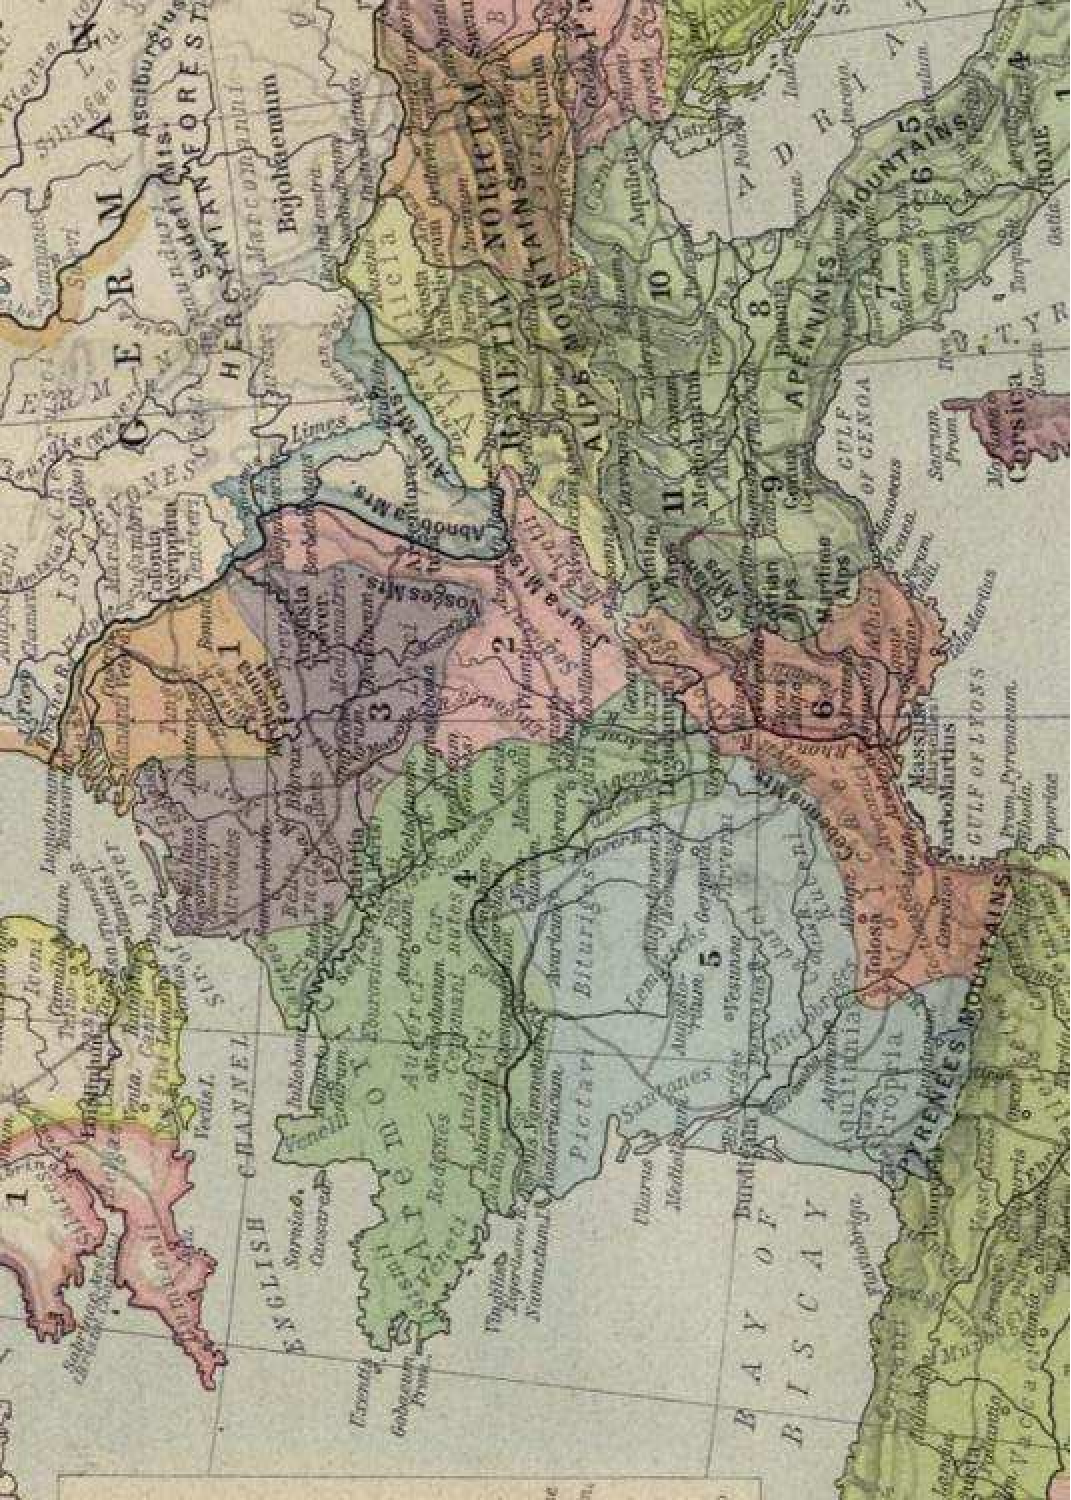
\includegraphics[width=175pt, angle=270]{bilder/Galia}
  \caption{Gallien zur Zeit Caesars}\label{fig_Gallien}
\end{center}
\end{figure}


\begin{table}[htb]
\begin{center}
\begin{tabular}{|l|l|l|}
\hline
Jahr &  Erster Consul & Zweiter Consul\\
\hline \hline
1 & C. Caesar         & L. Aemilius Paullus\\
2 & P. Vinicius       & P. Alfenus Varus\\
3 & L. Aelius Lamia   & M. Servilius\\
4 & Sex. Aelius Catus &  C. Sentius Saturninus\\
5 & L. Valerius Messalla& Cn. Cornelius Cinna \\
suff. & C. Vibius Postumus &  C. Ateius Capito\\
6 & M. Aemilius Lepidus & L. Arruntius\\
\hline
\end{tabular}
 \caption{Römische Konsulen}\label{tab_Konsulen}
\end{center}
\end{table}


\pagebreak

\section{De Bello Hispaniensi}\raggedbottom 

Pharnace superato, Africa recepta, qui ex his proeliis cum
adulescente Cn. Pompeio profugissent, cum . . . et ulterioris
Hispaniae potitus esset, dum Caesar muneribus dandis in Italia
detinetur, . . . quo facilius praesidia contra compararet,
Pompeius in fidem uniuscuiusque civitatis confugere coepit. Ita
partim precibus partim vi bene magna comparata manu provinciam
vastare. Quibus in rebus non nullae civitates sua sponte auxilia
mittebant, item non nullae portas contra cludebant. Ex quibus si
qua oppida vi ceperat, cum aliquis ex ea civitate optime de Cn.
Pompeio meritus civis esset, propter pecuniae magnitudinem alia
qua ei inferebatur causa, ut eo de medio sublato ex eius pecunia
latronum largitio fieret. Ita pacis commoda hoste +hortato+
maiores augebantur copiae. +Hoc crebris nuntiis in Italiam missis
civitates contrariae Pompeio+ auxilia sibi depostulabant.

C. Caesar dictator tertio, designatus dictator quarto multis
+iterante diebus coniectis+ cum celeri festinatione ad bellum
conficiendum in Hispaniam cum venisset, legatique Cordubenses, qui
a Cn. Pompelo discessissent, Caesari obviam venissent, a quibus
nuntiabatur nocturno tempore oppidum Cordubam capi posse, quod nec
opinantibus adversariis eius provinciae potitus esset, simulque
quod tabellariis, qui a Cn. Pompeio dispositi omnibus locis
essent, qui certiorem Cn. Pompeium de Caesaris adventu facerent .
. . multa praeterea veri similia proponebant. Quibus rebus
adductus quos legatos ante exercitui praefecerat Q. Pedium et Q.
Fabium Maximum de suo adventu facit certiores, utque sibi
equitatus qui ex provincia fuisset praesidio esset. Ad quos
celerius quam ipsi opinati sunt appropinquavit neque, ut ipse
voluit, equitatum sibi praesidio habuit.

Erat idem temporis Sex. Pompeius frater qui cum praesidio Cordubam
tenebat, quod eius provinciae caput esse existimabatur; ipse autem
Cn. Pompeius adulescens Uliam oppidum oppugnabat et fere iam
aliquot mensibus ibi detinebatur. Quo ex oppido cognito Caesaris
adventu legati clam praesidia Cn. Pompei Caesarem cum adissent,
petere coeperunt uti sibi primo quoque tempore subsidium mitteret.
Caesar - eam civitatem omni tempore optime de populo Romano
meritam esse - celeriter sex cohortis secunda vigilia iubet
proficisci, pari equites numero. Quibus praefecit hominem eius
provinciae notum et non parum scientem, L. Vibiurn Paciaecum. Qui
cum ad Cn. P praesidia venisset, incidit idem temporis ut
tempestate adversa vehementique vento adflictaretur; aditusque vis
tempestatis ita obscurabat ut vix proximum agnoscere possent.
Cuius incommodum summam utilitatem ipsis praebebat. Ita cum ad eum
locum venerunt, iubet binos equites conscendere, et recta per
adversariorum praesidia ad oppidum contendunt. Mediisque eorum
praesidiis cum essent, cum quaereretur qui essent unus ex nostris
respondit, ut sileat verbum facere: nam id temporis conari ad
murum accedere, ut oppidum capiant; et partim tempestate impediti
vigiles non poterant diligentiam praestare, partim illo responso
deterrebantur. Cum ad portam appropinquassent, signo dato ab
oppidanis sunt reccepti, et pedites dispositi partim ibi
remanserunt, equites clamore facto eruptionem in adversariorum
castra fecerunt.

\pagebreak
\section{Weiteres Kapitel}\raggedbottom 
\subsection{Unterkapitel}
\subsection{Unterkapitel}
\end{comment}

\section{Grundlagen}\raggedbottom
\label{sec:Grundlagen}
In diesem Kapitel beschäftigen wir uns mit den theoretischen Grundlagen der Methoden, die benutzt wurden, um die Kundendaten zu analysieren. Dafür wollen wir zunächst die Syntax der Logfiles beschreiben.

\subsection{Syntax der Logeinträge}
\label{sub:Aufbau der Logeinträge}
Das IFP generiert bei seiner Benutzung mehrere verschiedene Logfiles. Je nach Art des Logfiles können hier verschiedene Informationen gespeichert werden wie z.B. Zeitstempel, UserIDs, Exception Messages usw. Da für diese Arbeit aber nur die sog. \glqq Sessionlogs\grqq{} relevant sind, soll auch nur deren Syntax beschrieben werden.\\
Die Einträge in den Sessionlogs spiegeln im Großen und Ganzen die Serveraktivität wider: Es werden ein- und ausgehende HTTP Requests festgehalten. Allerdings ist es nicht ausreichend nur eine Liste von Requests zu speichern. Sie müssen noch in einen gewissen Kontext gebracht werden. Deshalb werden zusätzlich zu den Requests auch Daten wie Zeitstempel, UserID, Parameter u.s.w. geloggt. Durch diese Informationen kann man nun nachvollziehen, welcher User zu welchem Zeitpunkt Daten gesendet bzw. angefragt hat. Neben der UserID wird auch die SessionID mit geloggt. Sobald sich ein User erfolgreich in das IFP einloggt, wird eine SessionID generiert. Diese SessionID ist vom Zeitpunkt des Logins bis zum Logout gültig. Möchte sich derselbe User nach dem Logout direkt noch einmal einloggen, wird eine neue SessionID generiert. Die folgende Abbildung zeigt die Requests, die beim Login Prozess geloggt werden: (ABB:LOGin-SESSIONLOG) (wahrscheinlicher besser im appendix)
\\
Man erkennt schnell, dass man die Einträge in den Logfiles grob in die folgenden Felder unterteilen kann:\\

\begin{center}
	\begin{tabular}{c}
		\begin{lstlisting}[numbers=none, basicstyle=\scriptsize,caption=Felder in Sessionlogs,captionpos=b,label=lst:tab_session_fields]
[Timestamp] [Loglevel] [SessionID] [CustomerID] [UserID] [TaskID] [HTTP Request]
		\end{lstlisting}
		%\label{lst:tab_session_fields}
	\end{tabular}
\end{center}

Da nun die Syntax der Einträge erkannt wurde, kann die Mustererkennung beginnen.


\subsection{Mustererkennung}
\label{sub:Mustererkennung}
	Generell kann man in vielen verschiedenen Medien Muster erkennen, wie z.B. Bilddateien, Musikdateien oder eben in Textdateien. Dabei kommt es im Wesentlichen darauf an, welche Muster man erkennen möchte. So könnte man einem Programm beibringen, bestimmte Fischarten auf Fotos zu erkennen \citep{DuHaSt01}. Ein allgemeiner Ansatz, das Problem der Mustererkennung zu lösen, ist es, das Problem in folgende Teilprobleme aufzuteilen (Zitat anderes buch):
\begin{enumerate}
	\item Segmentiereung
	\item Feature Extraction
	\item Klassifizierung
\end{enumerate}
An dieser Stelle wollen wir drauf hinweisen, dass diese Begriffe eher konzeptionell zu verstehen sind, anstatt wörtlich. Im Folgenden wollen wir dieses generelle Vorgehen auf die Einträge der Logfiles anwenden. 

\subsubsection{Segmentierung (bestimmung der relevanten felder)}
\label{ssub:Segmentierung}

In dem Schritt der Segmentierung wollen wir feststellen, welche Informationen aus den Logfiles für die Fragestellung relevant sind. Greifen wir dafür zunächst einmal die Definition aus der Einleitung auf, was es bedeutet ein Widget zu benutzen. Wie bereits erwähnt reicht ein pures Anzeigen von Informationen nicht aus; das Widget muss auch angeklickt werden. Ein Klick auf ein Widget hat i.d.R. immer denselben Effekt: man wird auf eine (evtl. vorgefilterte) Seite weitergeleitet. Das heißt, man sendet einen HTTP Request an den Server und der Server sendet eine Antwort. Also ist es offensichtlich, dass wir für unsere Analyse nur die HTTP Requests betrachten wollen und die Antworten des Servers irrelevant sind. Demnach sind wir nur an Einträgen interessiert, die in dem Feld [HTTP Request] aus Listing \ref{lst:tab_session_fields} mit \textit{Incoming Request} anfangen. Dadurch haben wir die Menge an Einträgen, die wir betrachten wollen, um ca. die Hälfte reduziert.\\
Betrachten wir nun den Rest des Feldes genauer anhand eines Beispieleintrags, in dem ein Widget benutzt wurde. Insbesondere die URL ist für uns von Interesse:\\
%\\
\begin{lstlisting}[style=base,numbers=none,caption = Beispiel URL,captionpos=b,label=lst:url-beispiel]
/MULTIVERSA-IFP/lightning/ecm/liquidity/banks/liquidity\_banks.jsf?selectedView=ecm.liquidity.banks.view.all\&viewType=0\&@widget=LiquidityByBanksWidgetContent@\&banks=RpBLVhy85c5u4nGKeISH0A\&conversationContext=3\&\_ns\_=f63a91bc-9ab1-472d-bcb0-b6771837ffaa3\&\_nc\_=
\end{lstlisting}
%\label{lst:url-beispiel}
%\\
%\\
Der Name des Widgets ist in der URL erkennbar, wie man hier rot markiert sehen kann.\\
Neben dem HTTP Request sind diese weiteren Felder von Relevanz:\\
\begin{itemize}
	\item Timestamp
	\item SessionID
	\item UserID
\end{itemize}

\subsubsection{Feature Extraction (transformation der daten)}
	\label{ssub:Feature_extraction}
Nachdem alle irrelevanten Daten in der Segmentierung eliminiert wurden, ist der nächste Schritt die feature extraction. Dieser Begriff könnte irreführend wirken, da in dieser Arbeit keine features im wörtlichen Sinn extrahiert werden, vielmehr werden die Daten in eine bestimmte Struktur transfomiert. Diese Struktur besteht aus drei Mengen, die Menge an Usern, die Menge an SessionIDs und die Menge an Widgets. Diese Struktur wird von nun an \textit{Session Entity} genannt. Eine Session Entity hat eine eindeutige UserID, eine eindeutige SessionID und eine Menge an Widgets, die in dieser Session benutzt wurden. Mit anderen Worten beinhaltet eine Session Entity die Informationen, welche Widgets in einer Session benutzt wurden. \redt{Abbildung X} soll diesen Zusammenhang verdeutlichen.\\
Zusätzlich zu der Information, welche Widgets benutzt wurden, wird noch festgehalten, zu welchem Zeitpunkt bzw. in welcher Reihenfolge sie benutzt wurden. Sowohl die Uhrzeit als auch die UserID werden im weiteren Verlauf der Arbeit keine tragende Rolle mehr spielen. Allerdings macht es Sinn diese Daten mit zu speichern, da sie für zukünftige Anwendungsfälle relevant werden können. In Kapitel (ENDE) wird dies genauer diskutiert.
%Prinzipiell gäbe es noch die Menge an time stamps, nach diesen wird aber nicht sortiert.

\subsubsection{Klassifizierung}
\label{ssub:Klassifizierung}
Nun da unsere Daten transformiert wurden können wir beginnen, die Daten zu klassifizieren. 
Da wir in Abschnitt \ref{sub:Problemstellung} verschiedene Fragen beantworten wollen, müssen wir dafür die Klassifizierung für diese beiden gesondert betrachten.
%\\
\subsubsubsection{Diagramm}\\
%\\
Um die Frage zu klären, wie sich die Widgetnutzung pro Tag verhält, wollen wir ein Linienhistogramm erstellen. Das hat den Vorteil, dass nicht nur die Nutzung an sich dargestellt wird, sondern auch ein Verlauf, bzw. ein Trend in der Nutzung der Widgets. Zusätzlich wird in einem Tortendiagramm die anteilige Widgetnutzung dargestellt werden.
%\\
\subsubsubsection{Assoziationsregeln}\\
%\\
Die Suche nach Assoziationsregeln wird auch oft als Warenkorbanalyse bezeichnet. Dabei geht es darum, in einer Datenbank Beziehungen zwischen den Daten zu finden. Bevor wir in die Theorie hinter den Assoziationsregeln eintauchen, wollen wir mit Hilfe der folgenden Tabelle die wichtigsten Begriffe vorstellen. Zum besseren Verständnis zeigen wir zu den Begriffen Analogien zu unserem Anwendungsfall und eines Online Shops.

\begin{table}[htb]
	\begin{center}
		\begin{tabular}{p{4cm}|l|p{5cm}}
			Allgemein & Online Shop & IFP\\
			%\hline
			%Datenbank & Die Menge aller Warenkörbe & Die Menge aller SessionIDs\\
			\hline
			Transaktion & Ein einzelner Warenkorb & Eine einzelne SessionID\\
			\hline
			Menge aller Transaktionen $D$ & Menge aller Warenkörbe $D$ & Menge aller SessionIDs $D$\\
			\hline
			Item & ein Produkt & ein Widget bzw. eine Widgetnutzung\\
			\hline
			Menge aller Items $I$ & Menge aller Produkte $I$ & Menge aller Widgets $I$
		\end{tabular}
		\caption{Begriffe zu Assoziationsregeln}
		\label{tab:begriffe_ar}
	\end{center}
\end{table}

	Nun wollen wir definieren, was eine Assoziationsregel ist. Betrachten wir dafür die Widgets $w_1$ und $w_2$. Eine Assoziationsregel wird mit \begin{equation*}w_1 \rightarrow w_2\end{equation*} notiert und sagt aus, dass wenn $w_1$ benutzt (also angeklickt) wurde, $w_2$ auch benutzt wurde. An eine Assoziationsregel sind zwei Werte geknüpft, die beschreiben, wie \glqq gut\grqq{} eine Regel ist: der \textit{Support} und die \textit{Konfidenz}. Diese Werte wollen wir mit Hilfe eines kleinen Beispiels definieren:\\

		\begin{table}[htb]
	\begin{center}
		\begin{tabular}{|l|l|}
			\hline
			SessionID&Benutzte Widgets\\ \hline
			1& $w_1,w_2,w_4,w_5$\\ \hline
			2& $w_1,w_3$\\ \hline
			3& $w_2,w_5$\\ \hline
			4& $w_1,w_2$\\ \hline
			5& $w_2,w_3,w_5$\\ \hline
		\end{tabular}
		\caption{Beispiel Datenbank zu Assoziationsregeln}
		\label{tab:bsp_ar}
	\end{center}
\end{table}

%\newpage
Wir wollen zunächst die Begriffe aus Tabelle \ref{tab:begriffe_ar} auf dieses Beispiel anwenden:
\begin{itemize}
	\item Tabelle \ref{tab:bsp_ar} ist unsere Datenbank
	\item Die Menge aller Items $I = \{w_1, w_2, w_3\}$. Eine Menge $X \subseteq I$ wird auch \textit{Itemset} genannt. Also wäre z.B. $\{w_1, w_3\} \subseteq I$ ein Itemset.
	\item Die Menge aller SessionIDs $D = \{1,2,3,4\}$. $T_i$ mit $i \in D$ und $T_i \subseteq I$. Demnach gilt z.B. $T_1 = \{w_1,w_2,w_3\}$
\end{itemize}

Der Support einer Menge wird definiert als:\\

\begin{equation*}
	\text{support(X)} = \frac{\text{Anzahl der Transaktionen, die X enthalten}}{\text{Anzahl aller Transaktionen}}, \text{ X} \subseteq I
\end{equation*}\\

Demnach gilt z.B. für X$_1$ =  $\{w_1,w_3\}$, X$_2$ = $\{w_2\}$ und X$_3$ = $\{w_1\}$:\\
\begin{equation*}
	\begin{split}
		\text{support(X$_1$)} = \frac{1}{5} = 0.2\\
		\\
		\text{support(X$_2$)} = \frac{4}{5} = 0.8\\
		\\
		\text{support(X$_3$)} = \frac{3}{5} = 0.6\\
	\end{split}
\end{equation*}

Also beschreibt der Support eines Itemsets die relative Häufigkeit des Itemsets im Bezug auf die Anzahl der Transaktionen in der Datenbank. Des Weiteren gilt für X,Y $\subseteq$ I:\\
\begin{equation*}
	\text{support(X $\rightarrow$ Y)} = \text{support(X $\cup$ Y)}
\end{equation*}

Als nächstes wollen wir die Konfidenz definieren. Die Konfidenz einer Assoziationsregel X $\rightarrow$ Y definiert als:\\
\begin{equation*}
	\text{konfidenz(X $\rightarrow$ Y)} = \frac{\text{support(X $\rightarrow$ Y)}}{\text{support(X)}}
\end{equation*}

Auf unser Beispiel bezogen wollen wir nun die Konfidenz für die Regel $\{w_1\} \rightarrow \{w_2\}$ berechnen. Es gilt:\\
\begin{align*}
	\text{konfidenz($\{w_1\} \rightarrow \{w_3\}$)} &= \frac{\text{support($\{w_1\} \rightarrow \{w_3\}$)}}{\text{support($\{w_1\}$)}}\\ \\
	&= \frac{\text{support($\{w_1\} \cup \{w_3\}$)}}{\text{support($\{w_1\}$)}}\\ \\
	&= \frac{0.4}{0.6} = 0.67
\end{align*}
Die Konfidenz beschreibt also wie hoch die Wahrscheinlichkeit ist, dass wenn $w_1$ benutzt wurde, $w_3$ auch benutzt wurde. \citep{BeKe19}\\

Nachdem wir nun alle relevanten Begriffe bzgl. der Assoziationsregeln definiert haben, wollen wir genauer erörtern, wie Regeln gefunden werden sollen. Dazu rufen wir uns noch einmal ins Gedächnis, welche Information wir uns aus den Regeln erhoffen: wir wollen Workflows erkennen. Nehmen wir mal an, das Itemset $\{w_1,w_3\}$ käme in einer Datenbank mit 1000 Einträgen nur ein einziges Mal vor. Es ist offentsichtlich, dass man bei dieser Regel nicht von einem Workflow sprechen kann. Von daher suchen wir Itemsets, die \textit{häufig} vorkommen. Diese Häufigkeit wird durch den \textit{minsupport} festgelegt. Ein Itemset gilt als häufig, wenn gilt:\\
\begin{equation*}
	\text{support(X)} \geq \text{minsupport}
\end{equation*}

Analog wollen wir auch nicht alle Regeln, die wir aus den häufigen Itemsets generieren, betrachten. Vielmehr wollen wir die Regeln finden, die die \textit{minkonfidenz} erfüllen. Daraus folgt, dass wir unsere Aufgabe in zwei Teilprobleme aufteilen können:
\begin{enumerate}
	\item Finde alle Itemsets die häufig sind, also den minsupport erfüllen. Ein naiver Ansatz wäre, die Potenzmenge $\mathcal{P}$($I$) zu berechnen und zu prüfen, welche der Teilmengen den minsupport erfüllen. Allerdings hätte dieses Vorgehen eine Laufzeit von $\mathcal{O}(2^n)$ wobei n die Anzahl der Widgets ist. Deshalb wird der sog. \textit{Apriori Algorithmus} verwendet, der die Laufzeit stark einschränkt, indem die zu betrachtenden Itemsets eingeschränkt werden.\\
	\item Finde alle Assoziationsregeln, die aus den häufigen Itemsets generiert werden können und die die minkonfidenz erfüllen. Wenn Itemset X häufig ist, ist auch jede Teilmenge A von X häufig und ergibt die Regel A $\rightarrow$ X $-$ A. Für diese Regeln muss die Konfidenz geprüft werden.
\end{enumerate}

Bevor wir nun die Algorithmen vorstellen, die zu Lösung der Teilprobleme benutzt wurden, sei noch angemerkt, dass der minsupport und die minkonfidenz Werte sind, die vom Benutzter festgelegt sind.
%\\
\subsubsubsection{Apriori Algorithmus}\\
%\\
Der Apriori Algorithmus wurde von \citet{AgImSw93} entwickelt und wird benutzt, um möglichst effizient häufige Itemsets zu finden. Dabei wird folgendes Lemma ausgenutzt:
\begin{lemma}
	Sei X ein Itemset. Wenn X kein häufiges Itemset ist, ist auch keine Obermenge von X häufig. \citep{AgImSw93}
	\label{lem:sets}
\end{lemma}
Ausgangspunkt der Kandidatengenerierung ist, dass man häufige Itemsets mit $k$ Elementen betrachtet. Aus diesen Itemsets sollen nun Itemsets generiert werden, die $k+1$ Elemente beinhalten. Um das zu erreichen, werden zwei Itemsets vereinigt, die $k-1$ gleiche Elemente haben. Angenommen, wir hätten die häufigen Itemsets $X = \{w_1, w_2, w_3\}$ und $Y = \{w_1, w_2, w_4\}$. Beide Mengen haben $k=3$ Elemente. Um aus diesen Menge eine $k+1=4$ - elementige Menge zu generieren, müssen sie $k-1=2$ gleiche Elemente haben. Da das der Fall ist, erhalten wir als Ergebnis die Vereinigung beider Mengen mit $X \cup Y = \{w_1, w_2, w_3, w_4\}$. Dieser Schritt wird \textit{join} genannt.\\
Nach dem join muss noch geprüft werden, ob der generierte Kandidat auch Lemma \ref{lem:sets} erfüllt. Dies geschieht beim \textit{pruning} indem geprüft wird, ob jede $k-1$ - elementige Teilmenge des generierten Kandidaten ist. Denn wenn ein eine Teilmenge des generierten Kandidaten nicht häufig ist, kann dieser auch nicht häufig sein und muss nicht weiter betrachtet werden. In Anhang Teil \ref{anhang:zusatz1} wird die Kandidatengenerierung mit dem Beispiel aus Tabelle \ref{tab:bsp_ar} vorgerechnet.
%\\
\subsubsubsection{Assoziationsregeln finden}\\
%\\
Aus den häufigen Itemsets, die der Apriori Algorithmus gefunden hat, wollen wir nun Assoziationsregeln finden. Ähnlich wie bei den häufigen Itemsets wollen wir nur Regeln finden, die die minkonfidenz erfüllen. Dies erreichen wir, indem wir aus einem häufigen Itemset X zunächst Regeln bilden, die die Form 
\begin{equation*}
Y \rightarrow X - Y, Y \subset X
\end{equation*}
bilden. Ähnlich wie bei der Kandidatengenerierung nutzen wir wieder eine Teilmengenbeziehung aus: Wenn die Regel $Y \rightarrow X - Y$ die minkonfidenz nicht erfüllt, erfüllt auch keine Teilmenge $Y' \subset Y$ mit der Regel $Y' \rightarrow X - Y'$ die minkonfidenz.

\clearpage

\section{Umsetzung}
\label{sec:Umsetzung}

\subsection{Datengenerierung}
\label{sub:Datengenerierung}

Die zur Analyse genutzten Daten sind keine tatsächlichen Kundendaten, sondern wurden zum Zweck dieser Abschlussarbeit generiert.
Zur Generierung der Daten wurde ein Python Script benutzt. Das war notwendig, da in der aktuellen Version des IFPs die Widgetnamen nicht festgehalten werden und man in der aktuellen Implementierung nicht alle Widgets anhand der Logdateien erkennen kann. Selbst bei einer schnellen Auslieferung wäre der Zeitraum zu klein, um genügend Kundendaten zu sammeln. Mithilfe eines Python und Bash Scripts wurden zufällig generierte Logfiles für einen Zeitraum von X generiert. 

\subsection{Grundlagen zum Elastic Stack}
\label{sub:Grundlagen zum Elastic Stack}
Um die Fragen aus der Problemstellung zu beantworten, wurde der Elastic Stack (ELK) benutzt. Der ELK besteht aus den Software Produkten Elasticsearch, Logstash und Kibana von der Firma Elastic N.V. Zusätzlich wurde noch Filebeat von der gleichen Firma benutzt. Die Funktionen der einzelnen Produkte werden in den nachfolgenden Unterkapiteln weiter erläutert. Die folgende Abbildung stellt den Workflow des Systems dar:

\begin{figure}[htb]
\begin{center}
	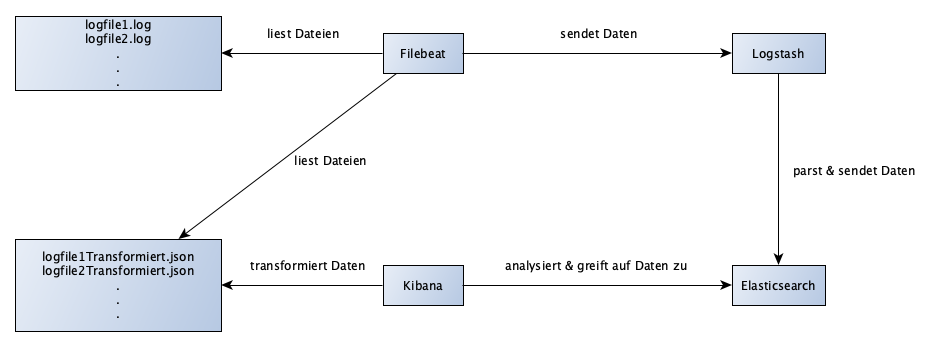
\includegraphics[width=440pt]{bilder/workflow.png}
\end{center}
\caption{ELK Workflow}
\label{fig:elk_workflow}
\end{figure}


\subsubsection{Filebeat}
\label{ssub:Filebeat}
Mit Filebeat können Dateien zeilenweise gelesen werden. In der Konfigurationsdatei von Filebeat gibt man an, wo und nach welchen Dateien gesucht werden soll. In unserem Fall waren es .log und .json Dateien. Außerdem kann man ein multiline pattern angeben, falls ein Eintrag mehrzeilig sein sollte. Die eingelesenen Dateien sendet Filebeat an Logstash weiter. Dabei merkt sich Filebeat, welche Dateien schon gelesen wurden und welche Zeilen in diesen Dateien gelesen wurden. Das bedeutet ebenfalls, wenn eine komplett neue Datei oder eine neue Zeile in einer alten Datei auftaucht, merkt Filebeat das, liest es und sendet die Daten wieder an Logstash. Damit ist die Echtzeitanalyse der Daten gewährleistet. 

\subsubsection{Logstash}
\label{sub:Logstash}
Die Aufgabe von Logstash ist es Daten von Filebeat zu empfangen und zu verarbeiten. Die empfangenen Daten befinden sich in einem rohen Zustand und werden mithilfe von mehreren Filter-Plugins verarbeitet. Nachdem die Daten verarbeitet wurden, sendet Logstash sie weiter an Elasticsearch.\\

\textbf{Grok Filter Plugin}\\
\\
Für die Logdateien wurde das Grok Filter-Plugin verwendet. In dem Grok-Filter gibt man einen regulären Ausdruck an, mitdem gematcht werden soll. Dabei kann man auch direkt festlegen, wie die Daten gespeichert werden sollen, falls gematcht wurde. Allgemein ist die Syntax dabei \%\{REGEXP:Feld\}. Neben einigen regulären Ausdrücken, die im Grok-Filter bereits implementiert sind (wie z.B. \textit{LOGLEVEL, TIMESTAMP\_ISO8601, SPACE, URIPATH}, uvm.) kann man auch eigene reguläre Ausdrücke definieren.
Wie schon in Kapitel \ref{ssub:Segmentierung} beschrieben, sollen die Daten segmentiert werden, was mit dem Grok-Filter realisiert werden kann. So kann man z.B. duch richtiges Platzieren von \textit{Incoming Request} in dem regulären Ausdruck erreichen, dass \textit{Outgoing Responses} nicht gematched und dadurch auch nicht weiter beachtet werden. Außerdem ist es möglich Daten matchen, aber keinem Feld zuweisen, wodurch sie auch nicht gespeichert werden. 
Die vollständige Konfiguration für die Logdateien sieht folgendermaßen aus:\\ (MACHE ICH DAS ÜBERHAUPT NOCH SO?)
\newpage
\begin{lstlisting}[caption = Sessionlog Filter,captionpos=b]
if [log][file][path] =~ "\S+session\S+" {
        grok{
            pattern_definitions => {
                "REQUEST" => "(Outgoing response|Incoming request)"
                "REQUEST_TYPE" => "(POST|GET)"
            }
            match => {"message" => [
                '^%{TIMESTAMP_ISO8601:zeit}%{SPACE}%{LOGLEVEL}%{SPACE}\[%{NOTSPACE:sessionid}\]\t\[%{NOTSPACE}\]\t\[%{NOTSPACE:userid}\]\t\[%{NOTSPACE} %{NOTSPACE}\]\t%{REQUEST:request}:%{SPACE}%{REQUEST_TYPE:request_type}%{SPACE}%{URIPATH:url}%{GREEDYDATA:stuff}',
                '^%{TIMESTAMP_ISO8601:zeit}%{GREEDYDATA:entry}'
                ]
            }
            remove_field => ['message']
        }

        if [url] !~ "\S+/rest" {
            drop{ }
        }

         mutate {
            gsub => [ "url", "\S+/rest", ""]
            remove_field => ['host','agent','@version','ecs','version']
        }

        date {
            match => [ "zeit", "ISO8601" ]
            target => "@timestamp"
		}

        if [request] == "Outgoing response"{
            drop { }
        }

        if [url] =~ "/fx/\S+" {
            mutate {
                gsub => ["url","/fx/\S+","/fx"]
            }
        }
\end{lstlisting}
\newpage
\label{lst:logEntryFilter}

\textbf{Ruby Filter Plugin}\\
\\
Das Ruby Filter Plugin wird benutzt, um transformierte Daten in Elasticsearch zu speichern. An dieser Stelle sei angemerkt, dass Elasticsearch zwar eine experimentelle \textit{transform} Funktion besitzt, diese aber für unseren Anwendungsfall (noch) nicht passend implementiert ist \citep{ElTr20}. Deshalb wurde ein Ruby Skript entwickelt, das diese Funktion ergänzt.\\

Die Daten, die nach dem Gedanken aus Abschnitt \ref{ssub:Feature_extraction} transformiert wurden, werden in einer JSON Datei gespeichert. Wie genau diese Daten aussehen bzw. wie sie zustande kommnen, wird in Kapitel \ref{ssub:Kibana} genauer erläutert. Zum besseren Verständnis, wie das Ruby Skript arbeitet, wird an dieser Stelle daher die Datenstruktur abstrakt beschrieben.
Im Prinzip sind die Daten in drei Ebenen aufgeteilt:\\
\begin{enumerate}
	\item UserIDs
	\item SessionIDs
	\item Widgets
\end{enumerate}
Dabei kann man jeweils eine Ebene als ein Array betrachten. So besteht die oberste Ebene aus einem Array, das mit UserIDs gefüllt ist. Zu der UserID wird zusätzlich eine Array gespeichert, das aus SessionIDs besteht, die zu der UserID gehören. Zu diesen SessionIDs wird schließlich ebenfalls ein Array verknüpft, in dem festgehalten wird, welche Widgets in der Session genutzt wurden und wie oft. Nun durchläuft das Skript also die beschriebenen Array Ebenen und speichert die gegebenen Daten in passende Felder, die schließlich an Elasticsearch gesendet und dort in einem passenden Index gespeichert werden.

\subsubsection{Elasticsearch}
\label{ssub:Elasticsearch}
Nachdem die von Filebeat gelesenen Daten von Logstash geparst wurden, werden die Daten in Elasticsearch gespeichert. Dabei werden die Logeinträge und die transformierten Daten separat indiziert. Das bedeutet z.B., dass alle Einträge in den Logfiles vom 01.04.2020 und vom 02.04.2020 in eigenen Indizes gespeichert werden.

\subsubsection{Kibana}
\label{ssub:Kibana}
\textbf{Visualisierungen}\\
\\
Kibana ist ein Tool, um die Daten, die in Elasticsearch gespeichert sind, zu visualisieren bzw. zu analysieren. In Kibana werden schon einige Visualisierungmöglichkeiten mitgeliefert, von denen für diese Arbeit zwei benutzt wurden: die \textit{Pie} und \textit{Line} Visualisierungen. Erstere wurde benutzt um festzustellen, zu welchen Anteilen die zufälligen Widgeteinträge generiert wurden.\\
Die \textit{Line} Visualisierung wurde benutzt, um die erste Fragestellung aus \ref{sub:Problemstellung} zu beantworten. Die Visualisierung zeigt in einem zweidimensionalen Diagramm die Benutzung der Widgets über einen bestimmten Zeitraum, wobei dieser Zeitraum auf der x-Achse abgebildet wird. Die y-Achse gibt die Anzahl an Widget Nutzungen an. Das bedeutet ein Punkt in dem Diagramm zeigt an, wie oft ein Widget an einem bestimmten Tag benutzt wurde. Schließlich verbindet die Visualisierung die Punkte miteinander und so erhält man eine Linie, die der Widgetnutzung in einem bestimmten Zeitraum entspricht. Abbildung	\ref{fig:screen_lines} zeigt wie die Visualisierung beispielsweise aussehen könnte.

\begin{figure}[htb]
\begin{center}
	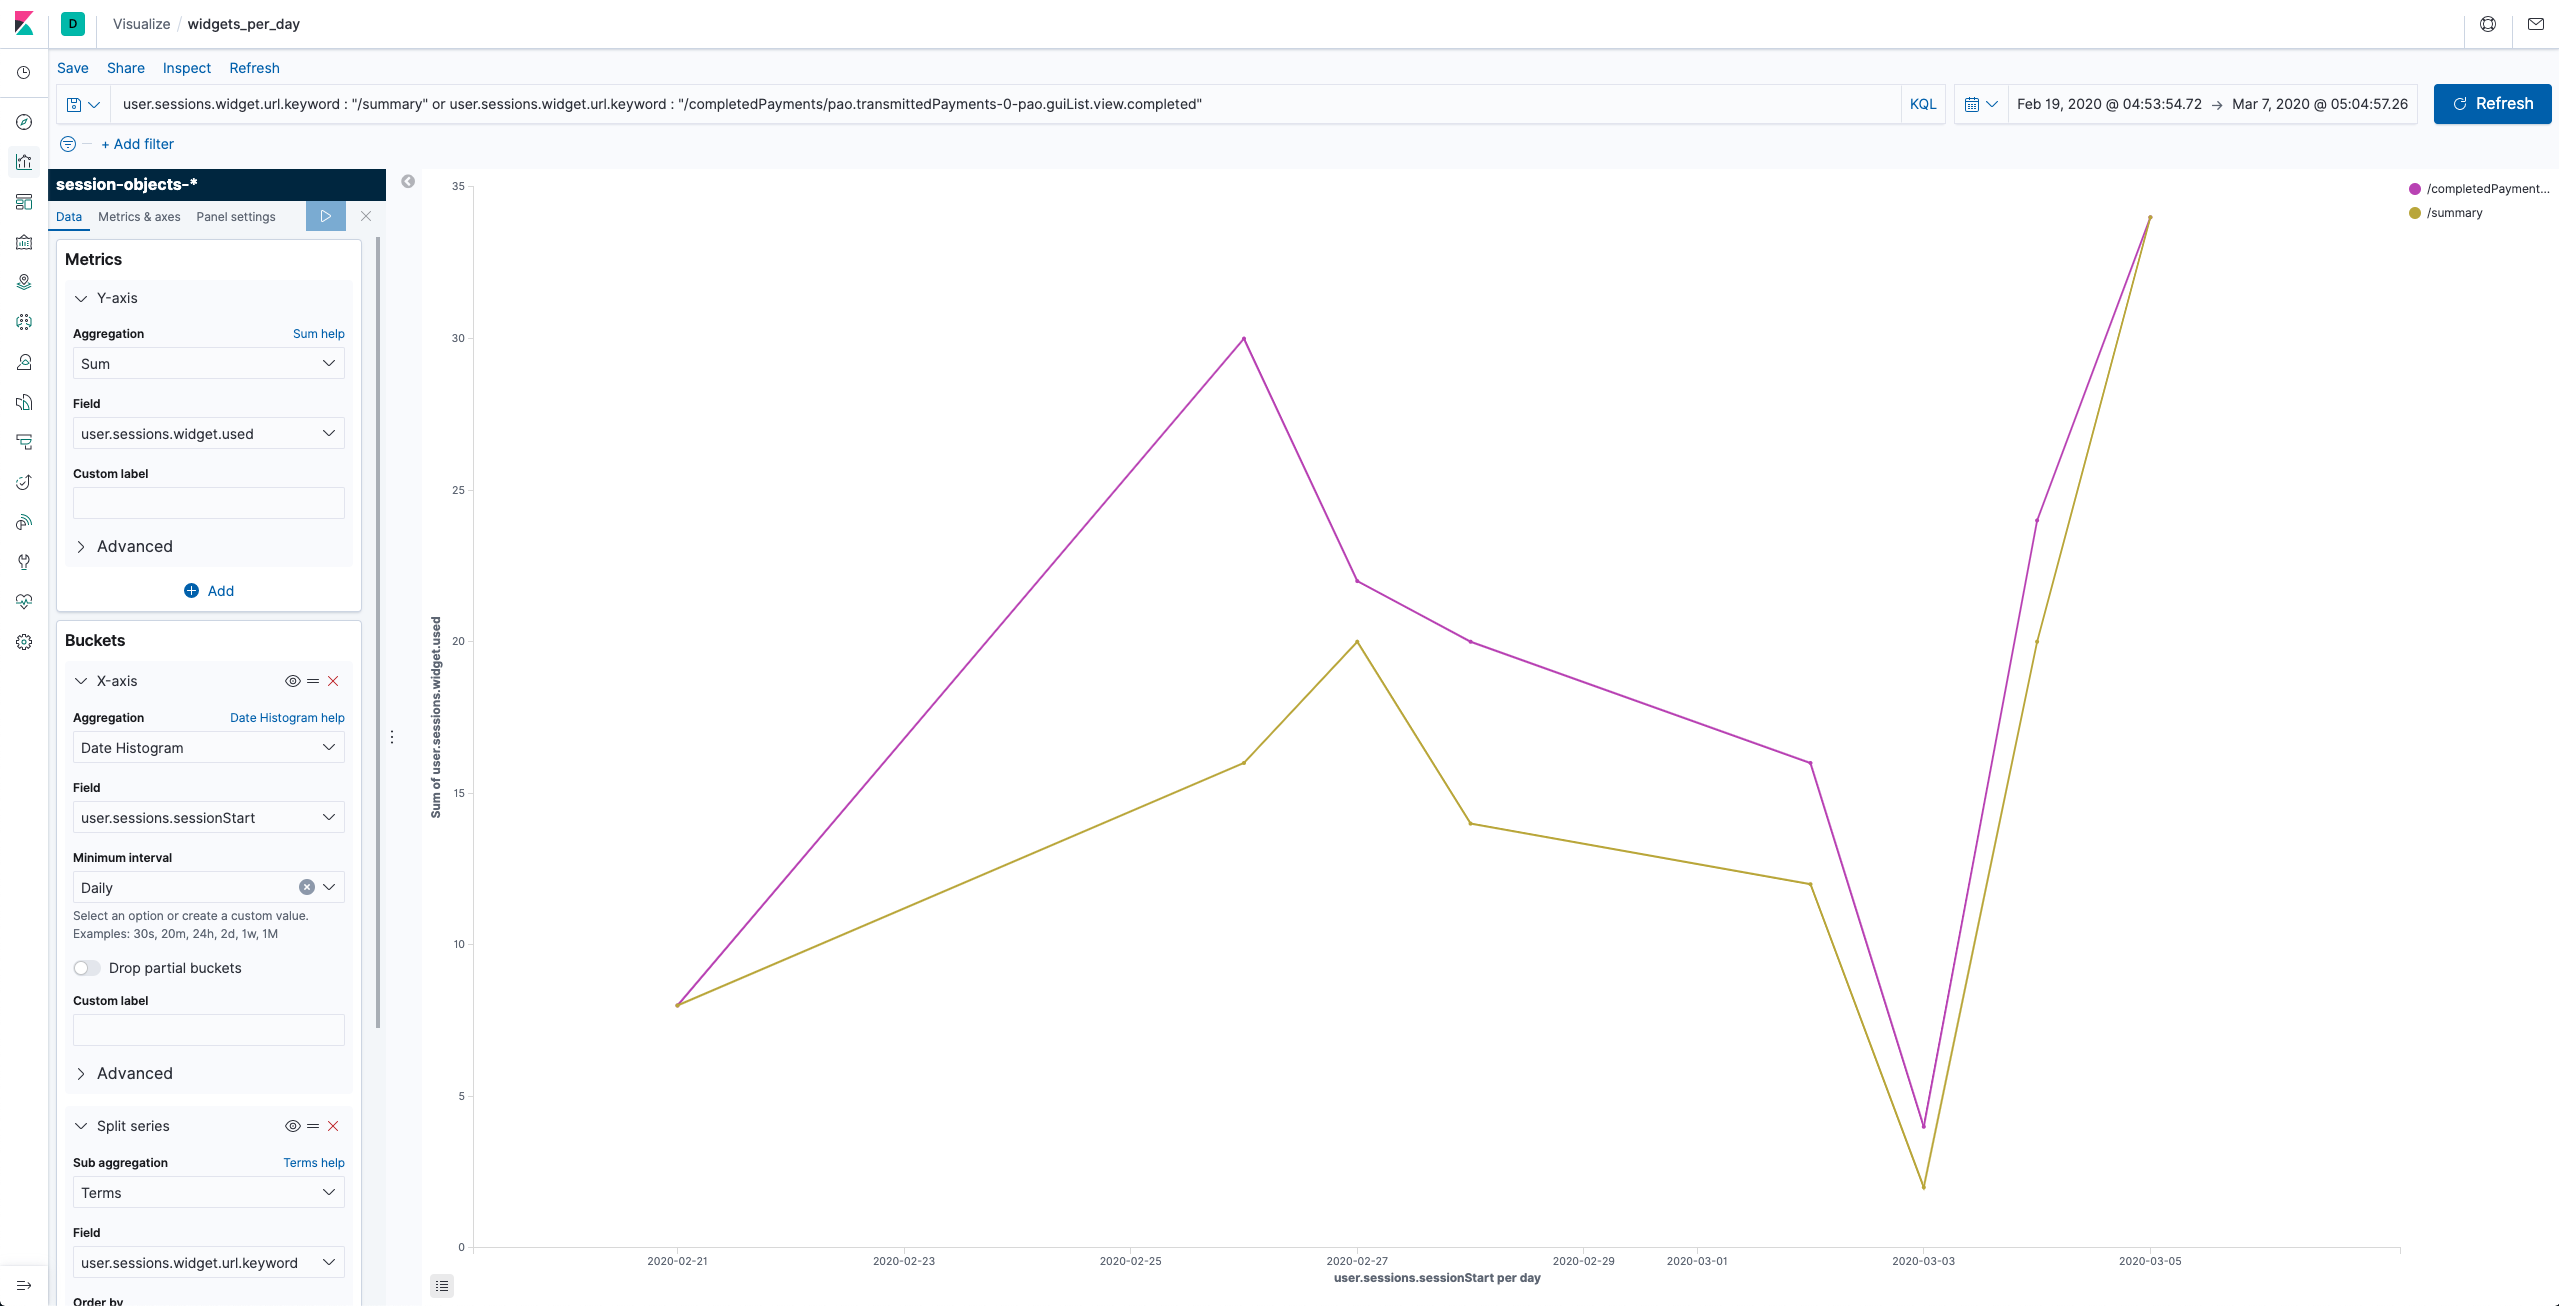
\includegraphics[width=430pt]{bilder/screen_lines.png}
\end{center}
\caption{Lines Visualisation mit zwei Widgets}
\label{fig:screen_lines}
\end{figure}

\textbf{Custom Plugin}\\\\
Kibana bietet aber nicht ohne Weiteres die Möglichkeit, einen Workflow zu erkennen, wie es in Kapitel \ref{sub:Problemstellung} gefordert ist. Deshalb würde im Zuge der Arbeit ein Custom Plugin für Kibana entworfen.

\section{Auswertung}
\label{sec:Auswertung}
In diesem Kapitel wird beschrieben, wie das entwickelte System eingesetzt und getestet wurde. Zuerst wird dargelegt, mit welchen Daten das System getestet wird. Als nächstes wird der Ablauf zur Durchführung des Tests beschrieben. Eine kritische Beleuchtung der Ergebnisse schließt das Kapitel ab.
\subsection{Datengenerierung}
\label{sub:Datengenerierung}

Die zur Analyse genutzten Daten sind keine tatsächlichen Kundendaten, sondern wurden zum Zweck dieser Abschlussarbeit generiert. Das war notwendig, da in der aktuellen Version des IFPs die Widgetnamen in der URL nicht festgehalten werden. Dadurch ist es nicht möglich, die Widgets anhand der URL eindeutig zu bestimmen. Selbst bei einer schnellen Auslieferung wäre der Zeitraum zu klein, um genügend Kundendaten zu sammeln.\\
Mithilfe eines Python Skripts wurden Logfiles für einen Zeitraum von 90 Tagen generiert. Die generierten Logfiles entsprechen einer verkürzten Version der normalen Logfiles: es wurden nur \textit{Incoming Requests} und Trennlinien, wie sie auch in den echten Logfiles vorkommen, in die generierten Dateien geschrieben. Zu Beginn der Entwicklung des Systems wurde der Logstash Filter mit Logfiles entworfen, in denen alle Einträge standen, also auch \textit{Outgoing Responses}. Zu diesem Zeitpunkt hat der Filter erfolgreich die Daten nach unseren Wünschen aus Kapitel \ref{ssub:Segmentierung} segmentiert. Deshalb war es für die Generierung der Daten ausreichend nur noch \textit{Incoming Requests} zu betrachten, die eine Widgetnutzung repräsentieren. Insgesamt wurden 15 verschiedene Widgets betrachtet.\\
Um zu prüfen, ob das entwickelte System nach unseren Wünschen funktioniert, müssen die Logfiles zwei Bedingungen erfüllen:\\
\begin{enumerate}
	\item Die Einträge in den Logfiles müssen zufällig ausgewählt werden. Die Idee hinter dieser Bedingung ist, dass die Daten in den Logfiles unbekannt sind.\\
	\item Eine Kombination an Widgets muss in verschiedenen Abständen wiederholt in den Logfiles vorkommen. Diese Kombination stellt einen bestimmten Workflow dar, der durch die Suche nach Assoziationsregeln erkannt werden soll. Die einzige Information, die wir zu diesem Punkt verwenden möchten, ist die Anzahl an Sessions und die Anzahl an Sessions, die diesen Workflow beinhalten. Durch diese Werte lässt sich der minsupport für den Workflow abschätzen und dient als Hilfe zur Erkennung des Workflows.
\end{enumerate}
Unter Berücksichtigung dieser Bedingungen wurde das Skript entwickelt. Eine Ausführung des Python Skripts entspricht einer Session. In dieser Session werden die Widgets, die \glqq benutzt\grqq{} werden, zufällig ausgewäht. Das wurde erreicht, indem die beispielhaften \textit{Incoming Requests} als Strings in einem Array gespeichert werden. Pythons \textproc{random} Funktion liefert eine zufällige Zahl in den Array Grenzen, die bestimmt welche Zeile geschrieben wird. Zusätzlich hat man die Möglichkeit bei der Ausführung des Skripts eine Reihe an Zahlen zu übergeben, die den Workflow darstellen. Schließlich kann über einen weiteren Parameter eine Zahl übergeben werden, die angibt welches Datum geloggt wird. Dieser Wert ist standardmäßig auf 0 gesetzt, was dem aktuellen Datum entspricht. Falls dieser Parameter übergeben wird, wird die Zahl zum aktuellen Datum addiert.\\
Zusätzlich zu dem Python Skript wurde ein Bash Skript entwickelt, welches die gesamte Datengenerierung automatisiert. Das Skript simuliert für einen festgelegten Zeitraum (in unserem Fall 30 Tage) eine zufällige Anzahl an Sessions pro Tag. Außerdem soll ca. jede dritte Session den festen Workflow beinhalten. Welche Widgets benutzt werden, wird durch drei zufällige Zahlen bestimmt. Am Ende gibt das Skript auf der Kommandozeile aus, wie viele Sessions insgesamt geschrieben wurden und wie viele davon den Workflow beinhalten.

\subsubsection{Durchführung}
\label{ssub:Durchführung}
Als erstes wurde begonnen die Logfiles zu generieren, während dieses Vorgang wurde auch der ELK gestartet. Die Vorgänge laufen parallel ab, um den echten Anwendungsfall zu simulieren. Der echte Anwendungsfall ist, dass Daten geloggt werden während das IFP läuft, es aber auch schon Daten aus den vergangenen Tagen gibt. Nach der Generierung der Daten wird das Custom Plugin verwendet, um die Daten mithilfe des Pythonskripts zu transformieren. \\
Die transformierten Daten werden von Filebeat gelesen, von Logstash geparst und in den entsprechenden Indizes in Elasticsearch gespeichert. Damit sind die Daten für die Visualisierungen und die Suche nach Assoziationsregeln vorbereitet. \\
Um die Daten visualisieren zu können, muss man vorher in Kibana ein Index Pattern anlegen \citep{KibIndexPatt20}. Damit wird die Visualisierung aller Indizes berücksichtigt, die dem Pattern entsprechen. Um zu testen, ob die Transformierung erfolgreich war, werden zwei Pie Diagramme miteinander verglichen. Für die untransformierten Daten hat die Pie Visualisierung gezählt, wie oft ein Widget pro Index vorkommt und anteilig dargestellt. In den transformierten Daten haben wir die Information, wie oft ein Widget in einer Session benutzt wurde. Wenn man diesen Wert über alle Session Entities für ein Widget summiert und das gleiche Diagramm entsteht, zeigt das, dass die Daten korrekt transformiert wurden. In der Lines Visualisierung wird dann entsprechend die Summe der Nutzungen pro Tag aufgeführt.\\
Die Suche nach den Assoziationsregeln wird in dem Custom Plugin durchgeführt. Dazu wird der minsupport so gewählt, dass der festgelegte Workflow gefunden werden müsste. Der tatsächliche minsupport des Workflows kann auch höher sein als der vom Skript zu Datengenerierung errechnete, da auch per Zufall der Workflow in einer Session vorkommen kann. Es ist zu erwarten, dass wir Regeln erhalten, die eine Permutation des Workflows darstellen. Die Wahl der minkonfidenz entscheidet dabei, wie tief diese Permutation geht. Das bedeutet, dass man bei einem Workflow mit drei Widgets mindestens drei Regeln findet. In dem Custom Plugin kann man den minsupport und die minkonfidenz über ein Nummernfeld festlegen und per Buttonclick die Suche starten.\\
Zusätzlich zu den Ergebnissen der Suche wird eine Analyse des Speicherverbrauchs des Skripts durchgeführt, mit Fokus auf die Funktionen zur Bestimmung der häufigen Itemsets und der Generierung der Regeln. Dazu wird das Python Modul \mbox{\textproc{memory\_profiler}} \citep{PeGe20} benutzt. Hierbei werden vier Szenarien analysiert, die sich in der Festlegung des minsupports und der minkonfidenz unterscheiden.

\subsubsection{Resultate}
\label{ssub:Resultate}
An dieser Stelle werden die Resultate nach der Durchführung aus Kapitel \ref{ssub:Durchführung} dargestellt.
Dazu werden zunächst die Pie Diagramme (Abbildung \ref{fig:generated-pie} und Abbildung \ref{fig:transformed-pie}) in Anhang Teil \ref{anhang:zusatz2} vorgestellt. Wie man erkennen kann, sind die beiden Diagramme identisch. Das bedeutet, dass die Lines Visualisierung aus Kapitel \ref{ssub:Kibana} den Verlauf der Widgetnutzung korrekt darstellt.\\
Wenden wir uns nun den Assoziationsregeln zu. Das Skript zur Generierung der Daten hat insgesamt 914 Sessions geschrieben, wovon 275 Sessions einen festen Workflow enthalten. Somit ergibt sich ein minsupport von mindestens 0.30 \footnote{Der tatsächliche minsupport der Regel kann auch höher sein, da das Itemset auch zufällig in einer Session vorkommen kann}. Als minkonfidenz wurde 0.80 gewählt. Abbildung \ref{fig:associationrule-result} zeigt welche Regeln gefunden wurden:\\
\begin{figure}[htb]
\begin{center}
	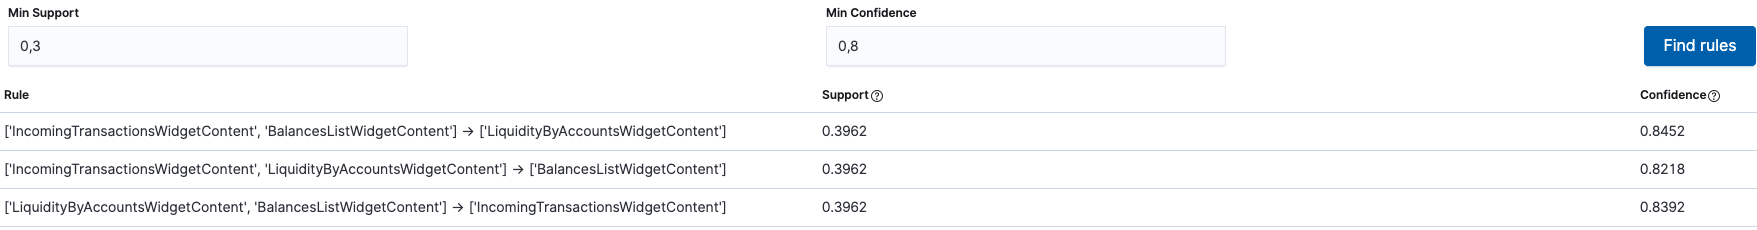
\includegraphics[width=430pt]{bilder/associationrules_result.png}
\end{center}
\caption{Ergebnis der Suche nach Assoziationsregeln}
\label{fig:associationrule-result}
\end{figure}
\\
Wie sich erkennen lässt, tritt das Itemset \textit{IncomingTransactionWidgetContent, BalancesWidgetContent} und \textit{LiquidityByAccountsWidgetContent} bzgl. des angegebenen minsupports häufig auf. Desweiteren stellen die Regeln eine Permutation dar, in der jedes Widget ein Mal als Konsequenz vorkommt. Daraus lässt sich ableiten, dass die Implementierung zum Finden der Assoziationsregeln korrekt funktioniert.\\
Aus der Analyse des Speicherverbrauchs resultieren die folgenden Plots:\\
\clearpage
\begin{figure}[htb]
\begin{center}
	\begin{subfigure}{0.47\textwidth}
		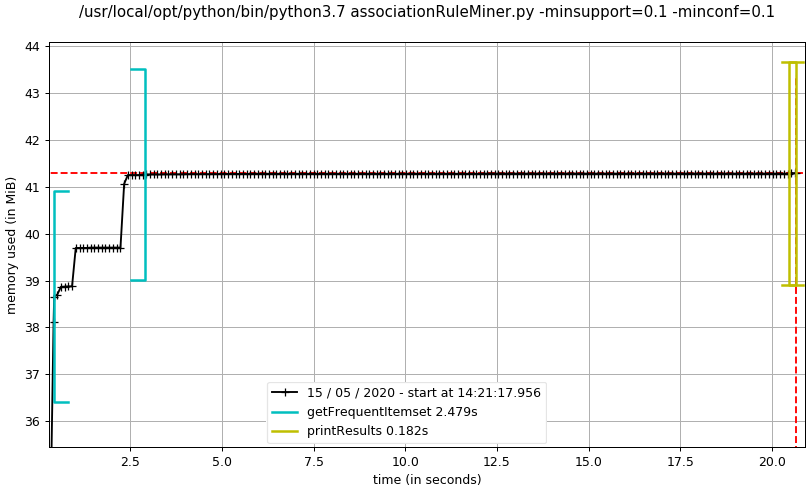
\includegraphics[width=\textwidth]{bilder/ass-conf-0101.png}
		\caption{}
		\label{subfig:0101}
	\end{subfigure}\qquad
	\begin{subfigure}{0.47\textwidth}
		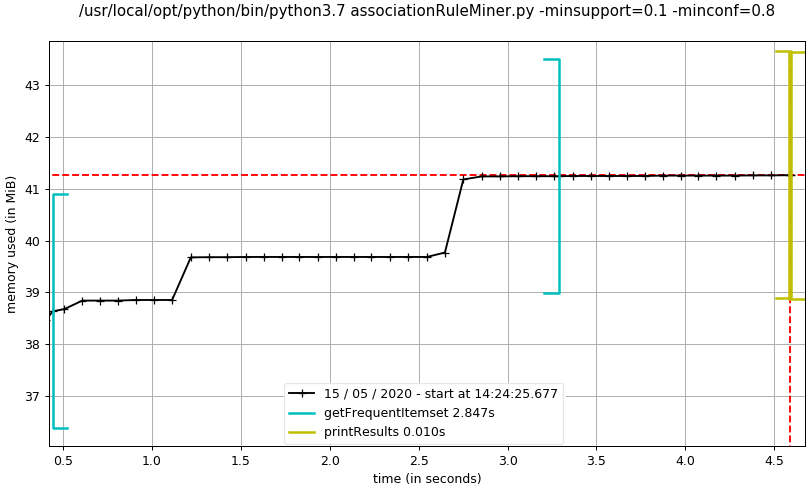
\includegraphics[width=\textwidth]{bilder/ass-conf-0108.png}
		\caption{}
		\label{subfig:0108}
	\end{subfigure}\\
	\begin{subfigure}{0.47\textwidth}
		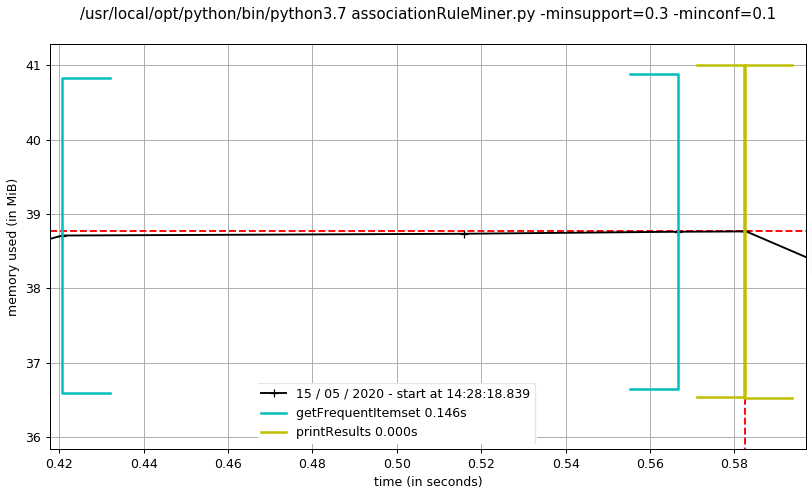
\includegraphics[width=\textwidth]{bilder/ass-conf-0301.png}
		\caption{}
		\label{subfig:0301}
	\end{subfigure}\qquad
	\begin{subfigure}{0.47\textwidth}
		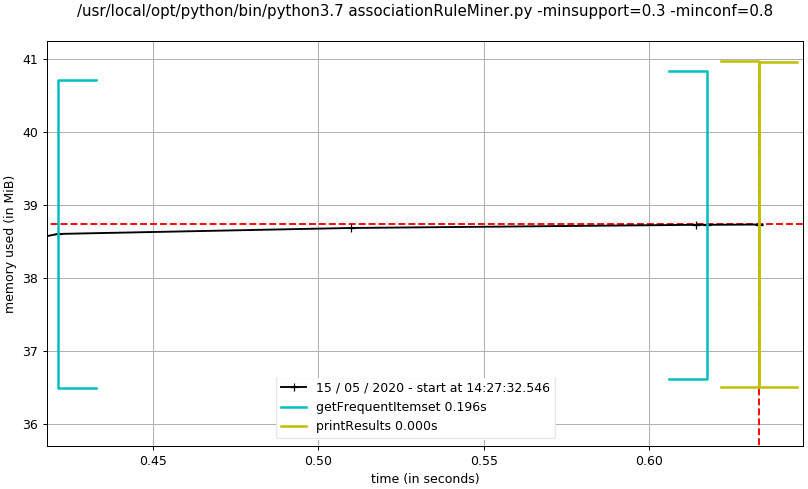
\includegraphics[width=\textwidth]{bilder/ass-conf-0308.png}
		\caption{}
		\label{subfig:0308}
	\end{subfigure}
\end{center}
\caption{Ergebnis Speicheranalyse}
\label{fig:result-mem-analysis}
\end{figure}
Die Plots zeigen den Speicherverbrauch ab dem Zeitpunkt, an dem die häufigen Itemsets bestimmt werden (blaue Klammer) bis zur Ausgabe der gefundenen Regeln (gelbe Klammer)\footnote{Für die Generierung der Assoziationsregeln wurde nicht direkt die Speichernutzung gemessen, sondern durch die Funktionen getFrequentItemsets und printResults eingegrenzt. Diese Funktionen werden unmittelbar vor bzw. nach der Generierung der Regeln aufgerufen. Der Grund für diese Vorgehensweise ist, dass \textproc{memory\_profiler} pro Funktionsaufruf eine Klammer darstellt. Da die Regeln rekursiv gefunden werden, wären zu viele Klammern in dem Plot erschienen, was die Lesbarkeit stark einschränkt.} an. Der Bereich zwischen den Klammern stellt den Speicherverbrauch während der Generierung der Regeln dar. Die Parameter für die Werte minsupport und minkonfidenz wurden so gewählt, dass sie einmal einen eher schlecht gewählten Wert bekommen (0.1) und entsprechend passendere Werte (minsupport = 0.3, minkonfidenz = 0.8). Es ist trivial, dass sich der gewählte minsupport auf die blaue Klammer auswirkt und die minkonfidenz auf die gelbe Klammer. Allerdings wirkt sich ein unpassend gewählter minsupport vergleichsweise stark auf die Speichernutzung aus. Vergleichen wir dazu einmal Abbildung \ref{subfig:0108} und Abbildung \ref{subfig:0308}. Wie sich deutlich erkennen lässt, wird bei einem niedrigen minsupport wesentlich mehr Speicher benötigt, da mehr Kandidaten für häufige Itemsets betrachtet werden müssen. Dementsprechend dauert es auch länger alle häufigen Itemsets zu bestimmen. Betrachtet man den Bereich zwischen der blauen und gelben Klammer, der die Generierung der Regeln darstellt, lässt sich festestellen, dass sich die Wahl der minkonfidenz mehr auf die benötigte Zeit auswirkt, um Regeln zu finden, als auf die Speichernutzung. Das sieht man besonders, wenn man Abbildung \ref{subfig:0101} und Abbildung \ref{subfig:0108} miteinander vergleicht: im ersten Fall müssen wesentlich mehr Funktionsaufrufe getätigt werden, erkennbar an den schwarzen, senkrechten Strichen auf der schwarzen Linie.

\subsubsection{Diskussion}
\label{ssub:Diskussion}
In diesem Abschnitt sollen die Ergebnisse aus Kapitel \ref{ssub:Resultate} kritisch diskutiert werden.\\
Wenden wir uns dazu zunächst den Visualisierungen zu. Anscheinend ist es für die Visualisierung nicht zwingend notwendig, die Daten zu transformieren. Das folgt aus der Tatsache, dass es Möglich war, das selbe Diegramm aus zwei verschiedenen Indices zu erstellen.\\
Dennoch hat die Transformierung den Vorteil, Daten in einem Format zu zeigen, welches sich für weitere Analyseverfahren in Bereich \textit{Knowledge Discovery in Databases} (KDD) eignet. Denkbar wäre hier die Anwendung der Nächste-Nachbarn-Klassifikation \citep{EsSa00} auf die Arrays, welche die Widgetnutzung pro Session speichern.\\
Im Bezug auf die Suche nach den Assoziationsregeln war es ebenfalls von Vorteil, die Daten transformiert zu betrachten. Durch die transformation hat ein besseres Verständnis über Daten erhalten.
%Mit Hilfe der Pie Diagramme wird gezeigt, dass die Daten richtig transformiert wurden und die Lines Visualisierung den Verlauf der Nutzung der Widgets ebenfalls korrekt darstellt. Daraus lässt sich schließen, dass für die Visualisierung an sich nicht zwingend notwendig ist, die Daten zu transformieren. Dennoch hat die Transformierung den Vorteil, dass die Daten in einem Format sind, das sich für weitere Analyseverfahren in Bereich \textit{Knowledge Discovery in Databases} (KDD) eignet. Denkbar wäre z.B. dass man auf die Arrays, die die Widgetnutzung pro Session speichern, die \textit{Nächste-Nachbarn-Klassifikation} \citep{EsSa00} anwendet.\\
\newline
Bevor die Ergebnisse der Assoziationsregelnanalyse diskutiert werden, ist es wichtig zu klären, welche Information eine Assoziationsregel genau liefert. Nach \citet{BeKe19} kann man den minsupport als relative Häufigkeit und die minkonfidenz als die Wahrscheinlichkeit einer Regel betrachten. Vergleichen wir dazu die erste Regel aus Abbildung \ref{fig:associationrule-result}. Diese Regel sagt aus, dass in 39.62\% aller Sessions die Widgets \textit{IncomingTransactionWidgetContent, BalancesWidgetContent} und \textit{LiquidityByAccountsWidgetContent} zusammen vorkommen. Mit einer Wahrscheinlichkeit von 84.52\% wird \textit{LiquidityByAccountsWidgetContent} angeklickt, wenn die anderen beiden Widgets benutzt wurden. Die Assoziationsregel suggeriert eine temporale Beziehung zwischen Antezedenz und Konsequenz der Regel. Tatsächlich berücksichtigt der in dieser Arbeit verwendete Algorithmus keine zeitlichen Aspekte, sodass dieser Rückschluss falsch sein kann \citep{Be03}.\\
Nichtsdestotrotz kann man bei realen Kundendaten vermuten, dass auch eine zeitliche Beziehung zwischen den Widgets besteht. Wird bspw. die Regel 
\begin{equation*}
\textit{Open Payments} \rightarrow \textit{LiquidityByAccountsWidgetContent} 
\end{equation*}
gefunden, die den minsupport und die minkonfidenz erfüllt, ist es naheliegend, dass \textit{Open Payments} zuerst benutzt wurde. Diese Interpretation basiert aber ausschließlich auf der Vermutung des Benutzers.\\
Aus dieser Feststellung folgt eine weitere Eigenschaft der Assoziationsregeln, die erwähnt werden muss. Da zeitliche Abfolgen nicht berücksichtigt werden, kann es auch durchaus sein, dass ein Workflow \glqq unterbrochen\grqq{} wird. Das bedeutet, dass zwischen der Antezedenz und Konsequenz einer Regel auch weitere Widgets benutzt worden sein können. Diese Tatsache wirkt zunächst wie eine Einschränkung für die Verwendbarkeit bzw. Aussagekraft der Assoziationsregeln. Man kann dies aber auch als Vorteil betrachten, da der Algorithmus Workflows trotz Unterbrechungen findet. So könnte eine Unterbrechung z.B. aus Versehen zustande kommen, indem sich ein User \glqq verklickt\grqq{} hat.\\
Mit Blick auf die Aufgabenstellung aus Kapitel \ref{sub:Problemstellung} lässt sich also zusammenfassen, dass die Suche nach Assoziationsregeln Workflows erkennen kann, mit der Voraussetzung, dass zeitliche Aspekte nicht berücksichtigt werden.
\clearpage

\section{Zusammenfassung}
\label{sec:Zusammenfassung}
In dem letzten Kapitel der Arbeit wird ein Fazit mit Blick auf die Ergebnisse aus dem vorherigen Kapitel gezogen. Schließlich werden zukünftige Anwendungsmöglichkeiten aufgezeigt, die sich auf drei Bereiche beziehen: Umwandlung, Optimierung und Erweiterung. In dem Abschnitt zur Umwandlung werden Denkansätze vorgestellt, wie man das System umwandeln kann, um es in neuen Bereichen einzusetzen. Anschließend geht es in dem Abschnitt zur Optimierung darum Stellen aufzuzeigen, welche ein Verbesserungspotential des entwickelten Systems bergen. Zum Schluss wird eine Aussicht auf Funktionalitäten gegeben, um die das System erweitert werden kann.
\subsection{Fazit}
\label{sub:Fazit}
Die Ergebnisse aus Kapitel \ref{sec:Auswertung} haben gezeigt, dass sich die im Rahmen dieser Arbeit vorgestellten Methoden durchaus eignen, Logfiles bzgl. des Userverhaltens zu analysieren. Trotzdem ist es wichtig an dieser Stelle anzumerken, dass die aktuelle Version des IFPs noch nicht die notwendigen Informationen in den Logfiles enthält und somit das System nicht direkt zur Analyse eingesetzt werden kann. Erst wenn in den Logfiles des IFPs bzw. in den URLs der Incoming Requests der Widgetname eindeutig festgehalten wird, ist dieses System einsetzbar. Es ist zwar durchaus möglich, einige Widgets anhand der Parameter in den URLs zu erkennen, aber damit würde man nur eine Teilmenge der Widgets abdecken, die zum Einsatz kommen.\\
Ebenso sei an dieser Stelle erwähnt, dass die Mittel und Wege zur Datenanalyse in dieser Arbeit nur eine mögliche Variante sind, an das erwünschte Ziel zu kommen. Während der Umsetzung der technischen Aspekte der Arbeit, wurden mehrere Ansätze ausprobiert die gegebenen Probleme zu lösen. Als Beispiel lässt sich das Ruby Filter-Plugin aus Kapitel \ref{sub:Logstash} nennen. Anstelle des hier angewendeten Plugins kan man auch das JSON Filter-Plugin benutzen, um die transformierten Daten zu parsen. Da aber mit dem Ruby Filter-Plugin das gewünschte Ergebnis durch Ausprobieren schneller erreicht wurde, wurde dieses letzlich auch verwendet.

\subsection{Zukünftige Anwendungsmöglichkeiten}
\label{sub:Zukünftige Anwendungsmöglichkeiten}
Um diese Arbeit abzuschließen werden zukünftige Anwendungsmöglichkeiten vorgestellt. Zunächst werden Möglichkeiten vorgeschlagen, wie man die im Rahmen der Arbeit entwickelten Analysemöglichkeiten auf weitere Aspekte des IFPs umwandeln kann. Daran anknüpfend werden mögliche Optimierungen des System angeboten. Schließlich wird erläutert, wie man das System mit neuen Funktionalitäten erweitern könnte.
\subsubsection{Umwandlungen}
\label{ssub:Umwandlungen}

Wie bereits in Kapitel \ref{ssub:Diskussion} erwähnt, bietet sich durch die eingeführte Datenstruktur der Session Entities die Möglichkeit, vektorbasierte Analysen durchzuführen. Neben der Nächste-Nachbarn-Methode wäre es z.B. auch denkbar Widgets basierend auf der Häufigkeit der Nutzung zu klassifizieren. Eine solche Klassifikation kann man wiederum nutzen, um zu bestimmen, welche Widgets nicht so oft benutzt werden und damit auch nicht so beliebt sind. Basierend auf dieser Information besteht die Möglichkeit das Widget zu überarbeiten.\\

Bis jetzt wurde vorgestellt, wie man die Logfiles des IFPs nutzen kann, um das Kundenverhalten bzgl. der Widgetnutzung zu analysieren. Da das IFP aber einen größeren Funktionsumfang hat, ist es naheliegend die Analyse auf weitere Bereiche zu erweitern. Eine Möglichkeit wäre einen Workflow nicht nur auf Widgets zu beschränken, sondern alle Seiten, die in einer Session aufgerufen wurden, zu betrachten.

In Kapitel \ref{ssub:Diskussion} wurde bereits erörtert, dass die Assoziationsregelngenerierung keine zeitlichen Abfolgen berücksichtigt. Dies könnte man durch eine Modifikation des Algorithmus ändern. \citep{Be03}\\
Desweiteren wäre es auch denkbar, die Widgets in hierarchische Strukturen einzuteilen und diese bei der Analyse zu berücksichtigen. Man könnte den Algorithmus auch dahingehend modifizieren, dass die Quantität der Widgets berücksichtigt wird \citep{EsSa00}\\
\subsubsection{Optimierung}
\label{ssub:Optimierung}
An dieser Stelle sei drauf hingewiesen, dass es zumindest einen Aspekt der Arbeit gibt, der in Zukunft optimiert werden sollte. In Kapitel \ref{ssub:Kibana} wurde erläutert, dass für die transformierten Daten zwei Indizes nötig seien, um die Visualisierungen darzustellen und die Datenstruktur der Session Entities akkurat in Elasticsearch zu speichern. Aus den Ergebnissen in Kapitel \ref{ssub:Diskussion} ist aber deutlich geworden, dass der extra Index für die Visualisierung der transformierten Daten redundant ist. Aus diesem Grund sollte in Zukunft darauf verzichtet werden, diesen Index anzulegen. Eine weitere Möglichkeit besteht darin, die transformierten Daten weder als JSON Dateien, noch in einem Index zu speichern. Stattdessen können die transformierten Daten temporär gecached werden. Es ist an dieser Stelle allerdings schwierig abzuschätzen, ob und wie vorteilhaft das wäre.
\subsubsection{Erweiterungen}
\label{ssub:Erweiterungen}
Abschließend wollen wir anregen, wie man das System um Funktionen erweitern kann, die von Elasticsearch angeboten werden. Da diese Möglichkeiten die kostenpflichtige Version von Elasticsearch voraussetzen, wurde im Rahmen dieser Arbeit zunächst darauf verzichtet, diese zu benutzen. So ist es sicherlich lohnenswert, sich Elasticsearchs Machine Learning Modul anzuschauen. Dort könnten ähnliche Analysemöglichkeiten enthalten sein, wie die im Kapitel \ref{ssub:Umwandlungen} vorgestellten \citep{ElMl20}.\\
Außerdem könnte die Alert Schnittstelle in Elasticsearch von Interesse sein. Mit dieser Erweiterung hat man die Möglichkeit Benachrichtigungen zu versenden, falls ein vom User definiertes Ereignis eintritt \citep{ElAl20}.

%%%%%%%%%%%%%%%%%%%%%%%%%%%%%%%%%%%%%%%%%%%%%%%%%%%%%%%%%%%%%%%%%%%%%%%%
%%%% ENDE TEXTTEIL %%%%%%%%%%%%%%%%%%%%%%%%%%%%%%%%%%%%%%%%%%%%%%%%%%%%%
%%%%%%%%%%%%%%%%%%%%%%%%%%%%%%%%%%%%%%%%%%%%%%%%%%%%%%%%%%%%%%%%%%%%%%%%

\clearpage

% Entfernen Sie das Kommentar aus der nachfolgenden Zeile, falls Sie einen Anhang in der Arbeit verwenden wollen. Beachten Sie, dass Sie sich im Verlauf der Arbeit mit \ref{...} (z.B. \ref{anhang:zusatz1}) auf den Anhang beziehen.
\newpage
\appendix
\section{Anhang}

\subsection*{Zusatzteil 1} \label{anhang:zusatz1}

Dies ist ein Anhang.

\clearpage

\ifthenelse{\boolean{\biber}}{ %with biber do
	\DeclareNameAlias{sortname}{first-last}
	\printbibliography[heading=bibintoc, title=\references]
}{ %without biber do
	\bibliography{references}
	\bibliographystyle{alphadin}
}
%\vspace*{\fill}

\clearpage

\listoffigures

\listoftables

\addcontentsline{toc}{section}{Listings}
\lstlistoflistings

%\pagebreak

%\printindex
\end{document}
